\newpage
\chapter*{\centering CHƯƠNG 4. HỆ THỐNG ĐỒ HỌA VÀ UI/UX}
\addcontentsline{toc}{chapter}{\textcolor{fitblue}{CHƯƠNG 4. HỆ THỐNG ĐỒ HỌA VÀ UI/UX}}
\setlength{\parindent}{1.5em}

\section*{4.1. Tổng quan pipeline đồ họa}
\addcontentsline{toc}{section}{\textcolor{black}{4.1. Tổng quan pipeline đồ họa}}

\setlength{\parindent}{1.5em} Chương này trình bày toàn bộ kiến trúc đồ họa và UI/UX của trò chơi, dựa trên cấu trúc triển khai và các mô-đun hệ thống. Hệ thống được xây dựng trên Win32 API kết hợp GDI/GDI+ theo hướng ``raster + procedural'', nhấn mạnh tốc độ, độ mượt và cảm giác thị giác retro \cite{ms_windows_gdi}. Phần này không chỉ mô tả cách vẽ mà còn lý giải các tối ưu quan trọng (double buffering, cache bitmap, palette động) và cách các màn hình thực tế ghép các thành phần đó thành trải nghiệm người dùng nhất quán.

\setlength{\parindent}{1.5em} Về mặt kỹ thuật, vòng đời đồ họa bắt đầu từ \texttt{InitGraphics} (khởi động GDI+), kế tiếp là \\ \texttt{GlobalFont::Initialize} để nạp font VT323, sau đó tạo \texttt{DoubleBuffer} để vẽ toàn bộ frame lên HDC bộ nhớ. Khi thoát game, \texttt{GlobalFont::Cleanup} gỡ font đã nạp và \texttt{ShutdownGraphics} giải phóng token GDI+ nhằm tránh rò rỉ tài nguyên hệ thống.

\setlength{\parindent}{1.5em} Pipeline hiển thị chia làm hai lớp:
\begin{itemize}
  \item \textbf{Lớp khởi tạo và tài nguyên toàn cục}: GDI+ được khởi tạo, font riêng (VT323) được nạp vào môi trường chạy, sau đó tạo các font theo tỉ lệ UI hiện tại.
  \item \textbf{Lớp vẽ theo khung hình}: các màn hình gọi renderer/utility để vẽ nền, panel, text, pixel art và hiệu ứng động. GDI được dùng cho các primitive đơn giản (text, line) trong khi GDI+ chịu trách nhiệm phần hiệu ứng và bitmap.
\end{itemize}

\setlength{\parindent}{1.5em} Các tệp cốt lõi trong RenderAPI gồm: \texttt{Renderer.*}, \texttt{UIScaler.*}, \texttt{Colours.*}, \texttt{UIComponents.*}. Những tệp này cung cấp API cấp cao để các mô-đun màn hình (\texttt{ScreenModule}) chỉ cần gọi hàm vẽ theo ngữ cảnh.

\setlength{\parindent}{1.5em} Luồng gọi chính vì vậy rất rõ ràng: mô-đun màn hình (\texttt{ScreenModule}) tính bố cục (theo \texttt{UIScaler}), gọi các hàm vẽ nền/đối tượng (trong \texttt{UIComponents}), sau cùng "đổ" nội dung ra màn hình thông qua buffer kép. Việc chia lớp giúp tránh trộn lẫn logic UI với xử lý tài nguyên mức thấp.

\section*{4.2. Renderer và tối ưu hóa hiển thị}
\addcontentsline{toc}{section}{\textcolor{black}{4.2. Renderer và tối ưu hóa hiển thị}}

\subsection*{4.2.1. Khởi tạo GDI+ và quản lý font}
\addcontentsline{toc}{subsection}{\textcolor{black}{4.2.1. Khởi tạo GDI+ và quản lý font}}

\setlength{\parindent}{1.5em} GDI+ được bật/tắt có kiểm soát, tránh rò rỉ tài nguyên. Font VT323 được load từ thư mục Asset và tạo 4 biến thể: Default, Bold, Title, Note. Điểm quan trọng là kích thước font phụ thuộc vào \texttt{UIScaler::S()}, đảm bảo phóng to/thu nhỏ đồng bộ với tỉ lệ màn hình.

\setlength{\parindent}{1.5em} Cụ thể, \texttt{AddFontResourceExW} dùng \texttt{FR\_PRIVATE} để font chỉ có hiệu lực trong tiến trình hiện tại, không ảnh hưởng hệ thống. Khi resize, \texttt{GlobalFont::RebuildFonts} xóa font cũ trước khi tạo mới, tránh leak GDI objects. Đây là phần quan trọng vì GDI giới hạn số handle, nếu không dọn đúng sẽ dẫn tới lỗi hiển thị sau thời gian dài.

\captionsetup{type=lstlisting}
\renewcommand{\arraystretch}{0.8}
\captionof{lstlisting}{Mã nguồn Khởi tạo font và tái tạo theo tỉ lệ UI}\label{lst:ch4_fonts}
\begin{longtable}{|>{\ttfamily\small\color{black}\raggedleft\arraybackslash}p{0.8cm}|>{\ttfamily\small\color{black}\arraybackslash}p{0.85\linewidth}|}
\hline
\normalfont\bfseries STT & \normalfont\bfseries Mã nguồn \\ \hline
1 & \cppkw{void} Initialize() \\ \hline
2 & \{ \\ \hline
3 & \ \ \textcolor{dkgreen}{// Nạp file Font từ thư mục Asset vào môi trường chạy tạm thời của Windows} \\ \hline
4 & \ \ AddFontResourceExW(L"Asset/font/VT323/VT323-Regular.ttf", FR\_PRIVATE, 0); \\ \hline
5 &  \\ \hline
6 & \ \ RebuildFonts(); \\ \hline
7 & \} \\ \hline
8 &  \\ \hline
9 & \cppkw{void} RebuildFonts() \\ \hline
10 & \{ \\ \hline
11 & \ \ \cppkw{if} (Default) \{ DeleteObject(Default); \} \\ \hline
12 & \ \ \cppkw{if} (Bold) \ \ \ \{ DeleteObject(Bold); \} \\ \hline
13 & \ \ \cppkw{if} (Title) \ \ \{ DeleteObject(Title); \} \\ \hline
14 & \ \ \cppkw{if} (Note) \ \ \ \{ DeleteObject(Note); \} \\ \hline
15 &  \\ \hline
16 & \ \ Default = CreateFontW(UIScaler::S(36), 0, 0, 0, FW\_NORMAL, FALSE, FALSE, FALSE, \\ \hline
17 & \ \ \ \ \ \ \ \ \ \ \ \ \ \ \ DEFAULT\_CHARSET, OUT\_DEFAULT\_PRECIS, CLIP\_DEFAULT\_PRECIS, \\ \hline
18 & \ \ \ \ \ \ \ \ \ \ \ \ \ \ \ NONANTIALIASED\_QUALITY, DEFAULT\_PITCH | FF\_DONTCARE, L"VT323"); \\ \hline
19 & \ \ Bold \ \ \ = CreateFontW(UIScaler::S(42), 0, 0, 0, FW\_BOLD, FALSE, FALSE, FALSE, \\ \hline
20 & \ \ \ \ \ \ \ \ \ \ \ \ \ \ \ DEFAULT\_CHARSET, OUT\_DEFAULT\_PRECIS, CLIP\_DEFAULT\_PRECIS, \\ \hline
21 & \ \ \ \ \ \ \ \ \ \ \ \ \ \ \ NONANTIALIASED\_QUALITY, DEFAULT\_PITCH | FF\_DONTCARE, L"VT323"); \\ \hline
22 & \ \ Title \ \ = CreateFontW(UIScaler::S(64), 0, 0, 0, FW\_HEAVY, FALSE, FALSE, FALSE, \\ \hline
23 & \ \ \ \ \ \ \ \ \ \ \ \ \ \ \ DEFAULT\_CHARSET, OUT\_DEFAULT\_PRECIS, CLIP\_DEFAULT\_PRECIS, \\ \hline
24 & \ \ \ \ \ \ \ \ \ \ \ \ \ \ \ NONANTIALIASED\_QUALITY, DEFAULT\_PITCH | FF\_DONTCARE, L"VT323"); \\ \hline
25 & \ \ Note \ \ \ = CreateFontW(UIScaler::S(28), 0, 0, 0, FW\_NORMAL, FALSE, FALSE, FALSE, \\ \hline
26 & \ \ \ \ \ \ \ \ \ \ \ \ \ \ \ DEFAULT\_CHARSET, OUT\_DEFAULT\_PRECIS, CLIP\_DEFAULT\_PRECIS, \\ \hline
27 & \ \ \ \ \ \ \ \ \ \ \ \ \ \ \ NONANTIALIASED\_QUALITY, DEFAULT\_PITCH | FF\_DONTCARE, L"VT323"); \\ \hline
28 & \} \\ \hline
\end{longtable}

\setlength{\parindent}{1.5em} Việc dùng \texttt{NONANTIALIASED\_QUALITY} giúp font giữ độ sắc và phù hợp phong cách pixel. Khi thay đổi kích thước cửa sổ, \texttt{UIScaler::Update()} sẽ cập nhật tỉ lệ, sau đó font được rebuild để đảm bảo tính nhất quán kích thước.

\subsection*{4.2.2. Double Buffering chống nhấp nháy}
\addcontentsline{toc}{subsection}{\textcolor{black}{4.2.2. Double Buffering chống nhấp nháy}}

\setlength{\parindent}{1.5em} Hiện tượng nhấp nháy (flicker) rất dễ xảy ra khi vẽ nhiều lớp. Để xử lý, renderer sử dụng bộ đệm kép: tạo một HDC bộ nhớ, vẽ toàn bộ frame lên đó, sau cùng mới blit ra màn hình. Tối ưu quan trọng là đảm bảo kích thước buffer tối thiểu 1x1 để tránh lỗi khi cửa sổ bị thu nhỏ.

\setlength{\parindent}{1.5em} Trong \texttt{CreateBuffer}, việc gọi \texttt{CreateCompatibleDC} và \texttt{CreateCompatibleBitmap} theo kích thước hiện tại giúp đảm bảo bề mặt vẽ tương thích với HDC cửa sổ. Sau khi tạo, buffer được xóa nền trắng bằng \texttt{FillRect} để tránh "rác" hình ảnh trong khung đầu tiên.

\captionsetup{type=lstlisting}
\renewcommand{\arraystretch}{0.8}
\captionof{lstlisting}{Mã nguồn Tạo bộ đệm kép theo kích thước cửa sổ}\label{lst:ch4_doublebuffer}
\begin{longtable}{|>{\ttfamily\small\color{black}\raggedleft\arraybackslash}p{0.8cm}|>{\ttfamily\small\color{black}\arraybackslash}p{0.85\linewidth}|}
\hline
\normalfont\bfseries STT & \normalfont\bfseries Mã nguồn \\ \hline
1 & \cppkw{void} CreateBuffer(HWND hwnd, HDC hdc, DoubleBuffer \&buffer) \\ \hline
2 & \{ \\ \hline
3 & \ \ RECT rect; \\ \hline
4 & \ \ GetClientRect(hwnd, \&rect); \\ \hline
5 & \ \ \cppkw{int} w = rect.right - rect.left; \\ \hline
6 & \ \ \cppkw{int} h = rect.bottom - rect.top; \\ \hline
7 &  \\ \hline
8 & \ \ \cppkw{if} (w <= 0) \{ w = 1; \} \\ \hline
9 & \ \ \cppkw{if} (h <= 0) \{ h = 1; \} \\ \hline
10 & \ \ buffer.width = w; \\ \hline
11 & \ \ buffer.height = h; \\ \hline
12 &  \\ \hline
13 & \ \ buffer.hdcMem = CreateCompatibleDC(hdc); \\ \hline
14 & \ \ buffer.hBitmap = CreateCompatibleBitmap(hdc, w, h); \\ \hline
15 & \ \ buffer.hOldBitmap = (HBITMAP)SelectObject(buffer.hdcMem, buffer.hBitmap); \\ \hline
16 &  \\ \hline
17 & \ \ RECT fillRect = \{0, 0, w, h\}; \\ \hline
18 & \ \ HBRUSH hBrush = CreateSolidBrush(RGB(255, 255, 255)); \\ \hline
19 & \ \ FillRect(buffer.hdcMem, \&fillRect, hBrush); \\ \hline
20 & \ \ DeleteObject(hBrush); \\ \hline
21 & \} \\ \hline
\end{longtable}

\subsection*{4.2.3. Đồng bộ resize và tái tạo back buffer}
\addcontentsline{toc}{subsection}{\textcolor{black}{4.2.3. Đồng bộ resize và tái tạo back buffer}}

\setlength{\parindent}{1.5em} Khi kích thước cửa sổ thay đổi, hệ thống cập nhật tỉ lệ UI, rebuild font và tái tạo back buffer để đảm bảo vùng vẽ luôn đúng kích thước. Cơ chế này đồng bộ trong xử lý \texttt{WM\_SIZE} để tránh tình trạng render vào buffer sai kích thước.

\setlength{\parindent}{1.5em} Việc \texttt{DeleteBuffer} luôn chọn lại \texttt{hOldBitmap} trước khi giải phóng nhằm tránh trạng thái HDC "treo" vào bitmap cũ. Đây là lỗi phổ biến trong GDI nếu không hoàn nguyên object trước khi \texttt{DeleteObject}.

\captionsetup{type=lstlisting}
\renewcommand{\arraystretch}{0.8}
\captionof{lstlisting}{Mã nguồn Cập nhật tỉ lệ và back buffer khi resize}\label{lst:ch4_resize_buffer}
\begin{longtable}{|>{\ttfamily\small\color{black}\raggedleft\arraybackslash}p{0.8cm}|>{\ttfamily\small\color{black}\arraybackslash}p{0.85\linewidth}|}
\hline
\normalfont\bfseries STT & \normalfont\bfseries Mã nguồn \\ \hline
1 & \cppkw{case} WM\_SIZE: \\ \hline
2 & \{ \\ \hline
3 & \ \ \cppkw{int} w = LOWORD(lParam); \\ \hline
4 & \ \ \cppkw{int} h = HIWORD(lParam); \\ \hline
5 & \ \ UIScaler::Update(w, h); \\ \hline
6 & \ \ GlobalFont::RebuildFonts(); \\ \hline
7 & \ \ HDC hdc = GetDC(hWnd); \\ \hline
8 & \ \ DeleteBuffer(g\_BackBuffer); \\ \hline
9 & \ \ CreateBuffer(hWnd, hdc, g\_BackBuffer); \\ \hline
10 & \ \ ReleaseDC(hWnd, hdc); \\ \hline
11 & \ \ InvalidateRect(hWnd, NULL, FALSE); \\ \hline
12 & \ \ \cppkw{return} DefWindowProc(hWnd, message, wParam, lParam); \\ \hline
13 & \} \\ \hline
\end{longtable}

\subsection*{4.2.4. GDI+ nâng cao: Alpha Blending và Linear Gradient}
\addcontentsline{toc}{subsection}{\textcolor{black}{4.2.4. GDI+ nâng cao: Alpha Blending và Linear Gradient}}

\setlength{\parindent}{1.5em} GDI+ được dùng để tạo các hiệu ứng thị giác ``mềm'' mà GDI thuần khó làm được: nền kính mờ (glassmorphism), viền phát sáng, gradient nền banner. Ví dụ \texttt{DrawPixelBanner} sử dụng \texttt{LinearGradientBrush} cho nền, thêm viền sáng theo nhịp sin để tạo cảm giác động.

\setlength{\parindent}{1.5em} Hàm \texttt{DrawPixelBanner} còn hỗ trợ icon pixel art ở hai đầu banner. Khi không cung cấp icon, hệ thống vẽ bóng (football) mặc định; khi có đường dẫn icon, hàm tự tạo palette động dựa trên màu nhấn của màn hình để đảm bảo icon hòa hợp với theme hiện hành.

\captionsetup{type=lstlisting}
\renewcommand{\arraystretch}{0.8}
\captionof{lstlisting}{Mã nguồn Banner gradient và viền pulse}\label{lst:ch4_banner_grad}
\begin{longtable}{|>{\ttfamily\small\color{black}\raggedleft\arraybackslash}p{0.8cm}|>{\ttfamily\small\color{black}\arraybackslash}p{0.85\linewidth}|}
\hline
\normalfont\bfseries STT & \normalfont\bfseries Mã nguồn \\ \hline
1 & Gdiplus::LinearGradientBrush gradBrush( \\ \hline
2 & \ \ Gdiplus::Point(bannerX, bannerY), \\ \hline
3 & \ \ Gdiplus::Point(bannerX + bannerW, bannerY), \\ \hline
4 & \ \ Gdiplus::Color(230, 10, 15, 25), \\ \hline
5 & \ \ Gdiplus::Color(230, 30, 60, 90)); \\ \hline
6 & g.FillRectangle(\&gradBrush, bannerX, bannerY, bannerW, bannerH); \\ \hline
7 &  \\ \hline
8 & \cppkw{float} pulse = 0.6f + sin(g\_GlobalAnimTime * 6.0f) * 0.4f; \\ \hline
9 & BYTE lineA = (BYTE)(180 + pulse * 75); \\ \hline
10 & Gdiplus::Pen topLine(Gdiplus::Color(lineA, gr, gg, gb), 2.5f); \\ \hline
11 & Gdiplus::Pen botLine(Gdiplus::Color((BYTE)(lineA * 0.6f), gr, gg, gb), 1.5f); \\ \hline
12 & g.DrawLine(\&topLine, bannerX, bannerY, bannerX + bannerW, bannerY); \\ \hline
13 & g.DrawLine(\&botLine, bannerX, bannerY + bannerH, bannerX + bannerW, bannerY + bannerH); \\ \hline
\end{longtable}

\setlength{\parindent}{1.5em} Nhờ alpha blending, các lớp kính và glow chồng lên nền sân vận động vẫn giữ độ rõ của nền phía sau, qua đó tạo chiều sâu cho UI.

\subsection*{4.2.5. Bitmap Caching cho đối tượng phức tạp}
\addcontentsline{toc}{subsection}{\textcolor{black}{4.2.5. Bitmap Caching cho đối tượng phức tạp}}

\setlength{\parindent}{1.5em} Các đối tượng vẽ bằng pixel art thường nặng nếu vẽ từng pixel mỗi frame. Hệ thống sử dụng nhiều cache độc lập:
\begin{itemize}
  \item \texttt{g\_RawModelCache}: cache dữ liệu ma trận số đọc từ file txt.
  \item \texttt{g\_ModelCache}: cache bitmap đã dựng từ ma trận + palette.
  \item \texttt{g\_AvatarCache, g\_ActionCache, g\_FootballCache, g\_TrophyCache, g\_ClockCache}: cache theo loại đối tượng.
  \item \texttt{g\_BrushCache}: cache các brush GDI+ theo màu ARGB để tránh new/delete liên tục.
\end{itemize}
\begin{table}[H]
\caption*{Bảng 4.1: Tổng hợp cache đồ họa và khóa nhận diện}
\addcontentsline{lot}{table}{Bảng 4.1: Tổng hợp cache đồ họa và khóa nhận diện}
\label{tbl:ch4_cache_map}
\centering
\renewcommand{\arraystretch}{0.9}
\begin{tabularx}{\linewidth}{|L{4.0cm}|L{4.2cm}|L{4.4cm}|X|}
\hline
\textbf{Cache} & \textbf{Dữ liệu} & \textbf{Khóa (key)} & \textbf{Ghi chú} \\ \hline
\texttt{g\_RawModelCache} & PixelModel thô & Đường dẫn file txt & Tránh đọc file lặp lại \\ \hline
\texttt{g\_ModelCache} & Bitmap từ model + palette & Hash (model ptr, size, palette) & Dùng lại bitmap đã dựng \\ \hline
\texttt{g\_AvatarCache} & Avatar bitmap & Hash (avatarType, size) & Fallback về avatar 0 nếu thiếu \\ \hline
\texttt{g\_ActionCache} & Action frame bitmap & Hash (avatarType, action, frame, flipH, size) & Cache theo từng frame hoạt họa \\ \hline
\texttt{g\_FootballCache} & Bitmap bóng & Size (int) & Vẽ pulse theo thời gian \\ \hline
\texttt{g\_TrophyCache} & Bitmap cúp & Size (int) & Dựng theo palette cúp \\ \hline
\texttt{g\_ClockCache} & Bitmap đồng hồ & Hash (size, color) & Màu phụ thuộc chủ đề \\ \hline
\texttt{g\_BrushCache} & GDI+ SolidBrush & ARGB value & Tránh new/delete liên tục \\ \hline
\end{tabularx}
\end{table}
\setlength{\parindent}{1.5em} Khi một model hoặc action đã được dựng, các frame sau chỉ cần vẽ lại bitmap đã cache bằng \texttt{DrawImage}, giảm đáng kể chi phí CPU.

\setlength{\parindent}{1.5em} Cơ chế cache dựa trên khóa hash (model pointer + size + palette) giúp hệ thống không cần ghép chuỗi tên file trong vòng lặp nóng. Điều này vừa tăng hiệu suất, vừa giảm phân mảnh bộ nhớ do tạo/huỷ string liên tục.

\section*{4.3. Pixel Art Engine}
\addcontentsline{toc}{section}{\textcolor{black}{4.3. Pixel Art Engine}}

\subsection*{4.3.1. Dựng hình từ ma trận dữ liệu số}
\addcontentsline{toc}{subsection}{\textcolor{black}{4.3.1. Dựng hình từ ma trận dữ liệu số}}

\setlength{\parindent}{1.5em} Pixel art được lưu dưới dạng file txt chứa kích thước và ma trận số (mỗi số là một mã màu). Ví dụ một file model được đọc bằng \texttt{LoadPixelModel} và dựng ảnh trong \texttt{DrawPixelModel}.

\setlength{\parindent}{1.5em} \texttt{LoadPixelModel} có cache cấp dữ liệu thô (\texttt{g\_RawModelCache}) để tránh đọc file lặp lại. Sau khi đọc, \texttt{model.isLoaded} được bật nhằm cho phép các bước dựng ảnh phía sau kiểm tra nhanh tính hợp lệ.

\begin{table}[H]
\caption*{Bảng 4.2: Kích thước các mô hình pixel art tiêu biểu}
\addcontentsline{lot}{table}{Bảng 4.2: Kích thước các mô hình pixel art tiêu biểu}
\label{tbl:ch4_pixel_models}
\centering
\renewcommand{\arraystretch}{0.9}
\begin{tabularx}{\linewidth}{|L{8.0cm}|L{3.0cm}|X|}
\hline
\textbf{File} & \textbf{Kích thước} & \textbf{Sử dụng} \\ \hline
\texttt{Asset/models/bg/title\_caro.txt} & 31\,$\times$\,8 & Tiêu đề banner Caro \\ \hline
\texttt{Asset/models/bg/badge.txt} & 12\,$\times$\,14 & Huy hiệu thắng \\ \hline
\texttt{Asset/models/bg/trophy.txt} & 12\,$\times$\,12 & Cúp tổng kết \\ \hline
\texttt{Asset/models/bg/clock.txt} & 8\,$\times$\,8 & Đồng hồ đếm ngược \\ \hline
\texttt{Asset/models/bg/cloud.txt} & 16\,$\times$\,6 & Mây nền sân \\ \hline
\texttt{Asset/models/bg/football.txt} & 8\,$\times$\,8 & Bóng khán đài \\ \hline
\texttt{Asset/models/avt\_00/avt.txt} & 48\,$\times$\,48 & Avatar cầu thủ \\ \hline
\end{tabularx}
\end{table}

\begin{table}[H]
\caption*{Hình 4.1: Hình minh họa dữ liệu pixel model (ví dụ title\_caro)}
\addcontentsline{lof}{figure}{Hình 4.1: Hình minh họa dữ liệu pixel model (ví dụ title\_caro)}
\centering

\includegraphics[width=0.9\linewidth]{images/ch4_pixel_model.png}
\end{table}

\setlength{\parindent}{1.5em} Ví dụ rút gọn nội dung file \texttt{Asset/models/bg/title\_caro.txt} (dòng đầu là kích thước, các dòng sau là ma trận mã màu):

\captionsetup{type=lstlisting}
\renewcommand{\arraystretch}{0.8}
\captionof{lstlisting}{Ví dụ file pixel art \texttt{title\_caro.txt}}
\label{lst:ch4_title_caro_txt}
\begin{longtable}{|>{\ttfamily\small\color{black}\raggedleft\arraybackslash}p{0.8cm}|>{\ttfamily\small\color{black}\arraybackslash}p{0.85\linewidth}|}
\hline
\normalfont\bfseries STT & \normalfont\bfseries Mã nguồn \\ \hline
1 & 31 8 \\ \hline
2 & 0 0 0 1 1 1 0 0 0 0 1 1 1 0 0 0 1 1 1 1 1 0 0 0 0 0 1 1 1 0 0 \\ \hline
3 & 0 0 1 2 2 2 1 0 0 1 2 2 2 1 0 0 1 2 2 2 2 1 0 0 0 1 2 2 2 1 0 \\ \hline
4 & 0 1 2 2 0 0 0 0 1 2 2 0 2 2 0 0 1 2 2 0 2 2 0 0 1 2 2 0 2 2 0 \\ \hline
5 & 0 1 2 2 0 0 0 0 1 2 2 2 2 2 0 0 1 2 2 2 2 1 0 0 1 2 2 0 2 2 0 \\ \hline
6 & 0 1 2 2 0 0 0 0 1 2 2 0 2 2 0 0 1 2 2 1 2 2 0 0 1 2 2 0 2 2 0 \\ \hline
7 & 0 0 1 2 2 2 1 0 1 2 2 0 2 2 0 0 1 2 2 0 2 2 0 0 0 1 2 2 2 1 0 \\ \hline
8 & 0 0 0 1 1 1 0 3 1 1 1 0 1 1 3 0 1 1 1 0 1 1 3 0 0 0 1 1 1 0 3 \\ \hline
9 & 0 0 0 0 3 3 0 0 0 3 3 0 0 3 0 0 0 3 3 0 0 3 0 0 0 0 0 3 3 0 0 \\ \hline
\end{longtable}

\captionsetup{type=lstlisting}
\renewcommand{\arraystretch}{0.8}
\captionof{lstlisting}{Mã nguồn Load dữ liệu pixel từ file txt}\label{lst:ch4_load_pixel}
\begin{longtable}{|>{\ttfamily\small\color{black}\raggedleft\arraybackslash}p{0.8cm}|>{\ttfamily\small\color{black}\arraybackslash}p{0.85\linewidth}|}
\hline
\normalfont\bfseries STT & \normalfont\bfseries Mã nguồn \\ \hline
1 & \cpptype{PixelModel} LoadPixelModel(const std::string \&filePath) \\ \hline
2 & \{ \\ \hline
3 & \ \ \cppkw{auto} it = g\_RawModelCache.find(filePath); \\ \hline
4 & \ \ \cppkw{if} (it != g\_RawModelCache.end()) \cppkw{return} it->second; \\ \hline
5 &  \\ \hline
6 & \ \ \cpptype{PixelModel} model; \\ \hline
7 & \ \ std::ifstream file(filePath); \\ \hline
8 & \ \ \cppkw{if} (!file.is\_open()) \{ \cppkw{return} model; \} \\ \hline
9 &  \\ \hline
10 & \ \ std::string line; \\ \hline
11 & \ \ \cppkw{if} (std::getline(file, line)) \{ \\ \hline
12 & \ \ \ \ std::stringstream ss(line); \\ \hline
13 & \ \ \ \ ss >> model.width >> model.height; \\ \hline
14 & \ \ \} \\ \hline
15 &  \\ \hline
16 & \ \ model.data.resize(model.height, std::vector<int>(model.width, 0)); \\ \hline
17 & \ \ \cppkw{for} (\cppkw{int} r = 0; r < model.height; ++r) \{ \\ \hline
18 & \ \ \ \ \cppkw{if} (!std::getline(file, line)) \cppkw{break}; \\ \hline
19 & \ \ \ \ std::stringstream ss(line); \\ \hline
20 & \ \ \ \ \cppkw{for} (\cppkw{int} c = 0; c < model.width; ++c) \{ \\ \hline
21 & \ \ \ \ \ \ \cppkw{int} val = 0; \\ \hline
22 & \ \ \ \ \ \ \cppkw{if} (ss >> val) model.data[r][c] = val; \\ \hline
23 & \ \ \ \ \} \\ \hline
24 & \ \ \} \\ \hline
25 & \ \ model.isLoaded = true; \\ \hline
26 & \ \ g\_RawModelCache[filePath] = model; \\ \hline
27 & \ \ \cppkw{return} model; \\ \hline
28 & \} \\ \hline
\end{longtable}

\setlength{\parindent}{1.5em} Quá trình dựng bitmap từ ma trận được tối ưu bằng hashing key (không dùng string concat trong vòng lặp nóng). Ngoài ra, mỗi pixel được vẽ kèm một đường lưới mờ để duy trì phong cách retro.

\setlength{\parindent}{1.5em} Trong \texttt{DrawPixelModel}, kích thước pixel \texttt{pSize} được suy ra từ \texttt{totalSize} và kích thước model, đảm bảo hình giữ đúng tỷ lệ. Khi vẽ, hệ thống đặt \texttt{InterpolationModeNearestNeighbor} và \texttt{PixelOffsetModeHalf} để tránh mờ biên, giữ đúng cảm giác pixel art.

\captionsetup{type=lstlisting}
\renewcommand{\arraystretch}{0.8}
\captionof{lstlisting}{Mã nguồn Dựng bitmap pixel art với cache và lưới}\label{lst:ch4_draw_model}
\begin{longtable}{|>{\ttfamily\small\color{black}\raggedleft\arraybackslash}p{0.8cm}|>{\ttfamily\small\color{black}\arraybackslash}p{0.85\linewidth}|}
\hline
\normalfont\bfseries STT & \normalfont\bfseries Mã nguồn \\ \hline
1 & size\_t key = (size\_t)\&model; \\ \hline
2 & hash\_combine(key, totalSize); \\ \hline
3 & \cppkw{for} (\cppkw{auto} \cppkw{const} \&[id, col] : palette) \\ \hline
4 & \{ \\ \hline
5 & \ \ hash\_combine(key, id); \\ \hline
6 & \ \ hash\_combine(key, col.GetValue()); \\ \hline
7 & \} \\ \hline
8 &  \\ \hline
9 & \cppkw{if} (g\_ModelCache.find(key) == g\_ModelCache.end()) \\ \hline
10 & \{ \\ \hline
11 & \ \ \cppkw{int} totalW = model.width * pSize; \\ \hline
12 & \ \ \cppkw{int} totalH = model.height * pSize; \\ \hline
13 & \ \ Gdiplus::Bitmap *bmp = \cppkw{new} Gdiplus::Bitmap(totalW + 2, totalH + 2, PixelFormat32bppARGB); \\ \hline
14 & \ \ Gdiplus::Graphics gBmp(bmp); \\ \hline
15 & \ \ gBmp.SetSmoothingMode(Gdiplus::SmoothingModeNone); \\ \hline
16 &  \\ \hline
17 & \ \ Gdiplus::Pen gridPen(Gdiplus::Color(60, 0, 0, 0), 1.0f); \\ \hline
18 & \ \ \cppkw{for} (\cppkw{int} r = 0; r < model.height; ++r) \\ \hline
19 & \ \ \{ \\ \hline
20 & \ \ \ \ \cppkw{for} (\cppkw{int} c = 0; c < model.width; ++c) \\ \hline
21 & \ \ \ \ \{ \\ \hline
22 & \ \ \ \ \ \ \cppkw{int} val = model.data[r][c]; \\ \hline
23 & \ \ \ \ \ \ \cppkw{if} (val != 0) \\ \hline
24 & \ \ \ \ \ \ \{ \\ \hline
25 & \ \ \ \ \ \ \ \ \cppkw{auto} it = palette.find(val); \\ \hline
26 & \ \ \ \ \ \ \ \ \cppkw{if} (it != palette.end()) \\ \hline
27 & \ \ \ \ \ \ \ \ \{ \\ \hline
28 & \ \ \ \ \ \ \ \ \ \ Gdiplus::SolidBrush *b = GetCachedBrush(it->second); \\ \hline
29 & \ \ \ \ \ \ \ \ \ \ gBmp.FillRectangle(b, c * pSize, r * pSize, pSize, pSize); \\ \hline
30 & \ \ \ \ \ \ \ \ \ \ gBmp.DrawRectangle(\&gridPen, c * pSize, r * pSize, pSize, pSize); \\ \hline
31 & \ \ \ \ \ \ \ \ \} \\ \hline
32 & \ \ \ \ \ \ \} \\ \hline
33 & \ \ \ \ \} \\ \hline
34 & \ \ \} \\ \hline
35 & \ \ g\_ModelCache[key] = bmp; \\ \hline
36 & \} \\ \hline
\end{longtable}

\setlength{\parindent}{1.5em} Hệ thống này cho phép các biểu tượng như bóng, cúp, đồng hồ, banner, mây, bóng bay được tạo hoàn toàn bằng dữ liệu (không cần PNG). Cách tiếp cận này giảm phụ thuộc vào asset ảnh, đồng thời cho phép thay đổi palette theo chủ đề một cách linh hoạt.

\subsection*{4.3.2. Palette và ngữ nghĩa màu}
\addcontentsline{toc}{subsection}{\textcolor{black}{4.3.2. Palette và ngữ nghĩa màu}}

\setlength{\parindent}{1.5em} Tệp \texttt{Colours.h} định nghĩa hai nhóm màu:
\begin{itemize}
  \item \textbf{Palette}: màu nguyên thủy dùng chung (đen, trắng, xám, đỏ, xanh, v.v.).
  \item \textbf{Theme}: màu ngữ nghĩa (shadow, glass panel, pitch, viền panel, màu P1/P2, highlight, v.v.).
\end{itemize}
\setlength{\parindent}{1.5em} Điểm nổi bật là bảng màu avatar có mã số riêng cho từng cầu thủ (Ronaldo, Messi, Neymar). Mỗi mã số (2,3,4,6,8,15,16...) được ánh xạ sang màu cụ thể để giữ nhận diện nhân vật.

\setlength{\parindent}{1.5em} Lớp màu được tách thành \texttt{Palette} (màu nguyên thủy) và \texttt{Theme} (màu ngữ nghĩa). Cấu trúc \texttt{SmartColor} là POD đơn giản để dễ copy/assign, còn chuyển đổi sang GDI/GDI+ được thực hiện qua \texttt{ToCOLORREF} và \texttt{ToGdiColor}. Cách này giúp toàn bộ pipeline màu nhất quán giữa GDI và GDI+.

\captionsetup{type=lstlisting}
\renewcommand{\arraystretch}{0.8}
\captionof{lstlisting}{Mã nguồn Bảng màu nguyên thủy và màu ngữ nghĩa}\label{lst:ch4_palette_theme}
\begin{longtable}{|>{\ttfamily\small\color{black}\raggedleft\arraybackslash}p{0.8cm}|>{\ttfamily\small\color{black}\arraybackslash}p{0.85\linewidth}|}
\hline
\normalfont\bfseries STT & \normalfont\bfseries Mã nguồn \\ \hline
1 & \cppkw{namespace} Palette \\ \hline
2 & \{ \\ \hline
3 & \ \ \cppkw{constexpr} \cpptype{SmartColor} Transparent = \{0, 0, 0, 0\}; \\ \hline
4 & \ \ \cppkw{constexpr} \cpptype{SmartColor} White = \{255, 255, 255, 255\}; \\ \hline
5 & \ \ \cppkw{constexpr} \cpptype{SmartColor} GrayDarkest = \{255, 33, 33, 33\}; \\ \hline
6 & \} \\ \hline
7 &  \\ \hline
8 & \cppkw{namespace} Theme \\ \hline
9 & \{ \\ \hline
10 & \ \ \cppkw{constexpr} \cpptype{SmartColor} GlassWhite = \{220, 255, 255, 255\}; \\ \hline
11 & \ \ \cppkw{constexpr} \cpptype{SmartColor} PanelBlueBorder = \{180, 0, 150, 255\}; \\ \hline
12 & \ \ \cppkw{constexpr} \cpptype{SmartColor} TitleFill = \{255, 255, 220, 0\}; \\ \hline
13 & \ \ \cppkw{constexpr} \cpptype{SmartColor} P1TurnPulse = \{30, 255, 150, 0\}; \\ \hline
14 & \} \\ \hline
\end{longtable}

\captionsetup{type=lstlisting}
\renewcommand{\arraystretch}{0.8}
\captionof{lstlisting}{Mã nguồn Tra mã màu avatar theo loại nhân vật}\label{lst:ch4_avatar_palette}
\begin{longtable}{|>{\ttfamily\small\color{black}\raggedleft\arraybackslash}p{0.8cm}|>{\ttfamily\small\color{black}\arraybackslash}p{0.85\linewidth}|}
\hline
\normalfont\bfseries STT & \normalfont\bfseries Mã nguồn \\ \hline
1 & \cppkw{static} \cpptype{SmartColor} LookupAvatarColor(\cppkw{int} type, \cppkw{int} code) \\ \hline
2 & \{ \\ \hline
3 & \ \ \cppkw{switch} (type) \\ \hline
4 & \ \ \{ \\ \hline
5 & \ \ \cppkw{case} 1: \textcolor{dkgreen}{// Messi} \\ \hline
6 & \ \ \ \ \cppkw{switch} (code) \\ \hline
7 & \ \ \ \ \{ \cppkw{case} 2: \cppkw{return} Theme::MES\_SkinL; \cppkw{case} 6: \cppkw{return} Theme::MES\_HairD; \} \\ \hline
8 & \ \ \cppkw{case} 2: \textcolor{dkgreen}{// Neymar} \\ \hline
9 & \ \ \ \ \cppkw{switch} (code) \\ \hline
10 & \ \ \ \ \{ \cppkw{case} 2: \cppkw{return} Theme::NEY\_SkinL; \cppkw{case} 13: \cppkw{return} Theme::NEY\_Shirt; \} \\ \hline
11 & \ \ \cppkw{default}: \textcolor{dkgreen}{// Ronaldo} \\ \hline
12 & \ \ \ \ \cppkw{switch} (code) \\ \hline
13 & \ \ \ \ \{ \cppkw{case} 2: \cppkw{return} Theme::CR7\_SkinL; \cppkw{case} 13: \cppkw{return} Theme::TitleFill; \} \\ \hline
14 & \ \ \} \\ \hline
15 & \ \ \cppkw{return} Theme::CR7\_SkinM; \\ \hline
16 & \} \\ \hline
\end{longtable}

\subsection*{4.3.3. Action Animation System}
\addcontentsline{toc}{subsection}{\textcolor{black}{4.3.3. Action Animation System}}

\setlength{\parindent}{1.5em} Hệ thống animation dùng thư mục hành động theo cấu trúc:
\begin{verbatim}
Asset/models/avt_00/idle/f_0.txt ...
Asset/models/avt_00/run/f_0.txt ...
Asset/models/avt_00/sad/f_0.txt ...
Asset/models/avt_00/win/f_0.txt ...
\end{verbatim}
\setlength{\parindent}{1.5em} Mỗi frame là một file txt. Hàm \texttt{DrawPixelAction} cập nhật frame theo thời gian, tạo cache key theo (avatar, action, frame, flip, size), fallback về frame 0 hoặc avatar mặc định khi thiếu dữ liệu.

\setlength{\parindent}{1.5em} Cụ thể, hệ thống dùng \texttt{GetTickCount64} để kiểm soát thời gian frame, đảm bảo animation ổn định kể cả khi FPS biến động. Khi thiếu frame, hàm tự reset về \texttt{f\_0.txt} và cập nhật cache key mới, giảm rủi ro crash do file không tồn tại. Việc hỗ trợ \texttt{flipH} giúp tái sử dụng sprite cho hai hướng di chuyển mà không cần thêm asset.

\begin{figure}[H] % Sử dụng figure thay vì table
    \centering
    \caption*{Hình 4.2: Hình minh họa chuỗi frame action run của avt\_00}
    \addcontentsline{lof}{figure}{Hình 4.2: Hình minh họa chuỗi frame action run của avt\_00}
    
    
\includegraphics[width=0.3\linewidth]{images/ch4_action_frames.png} \quad
    
\includegraphics[width=0.3\linewidth]{images/ch4_action_frames_2.png} \\[10pt] % Xuống hàng và tạo khoảng cách
    
    
\includegraphics[width=0.3\linewidth]{images/ch4_action_frames_3.png}
\end{figure}

\captionsetup{type=lstlisting}
\renewcommand{\arraystretch}{0.8}
\captionof{lstlisting}{Mã nguồn Cập nhật frame và dựng animation}\label{lst:ch4_action_anim}
\begin{longtable}{|>{\ttfamily\small\color{black}\raggedleft\arraybackslash}p{0.8cm}|>{\ttfamily\small\color{black}\arraybackslash}p{0.85\linewidth}|}
\hline
\normalfont\bfseries STT & \normalfont\bfseries Mã nguồn \\ \hline
1 & ULONGLONG now = GetTickCount64(); \\ \hline
2 & \cppkw{if} (now - state.lastFrameTime > (ULONGLONG)state.animationSpeed) \\ \hline
3 & \{ \\ \hline
4 & \ \ state.currentFrame++; \\ \hline
5 & \ \ state.lastFrameTime = now; \\ \hline
6 & \} \\ \hline
7 &  \\ \hline
8 & size\_t cacheKey = state.avatarType; \\ \hline
9 & hash\_combine(cacheKey, state.currentAction); \\ \hline
10 & hash\_combine(cacheKey, state.currentFrame); \\ \hline
11 & hash\_combine(cacheKey, state.flipH); \\ \hline
12 & hash\_combine(cacheKey, size); \\ \hline
13 &  \\ \hline
14 & std::string path = "Asset/models/avt\_0" + std::to\_string(state.avatarType) + \\ \hline
15 & \ \ \ \ \ \ \ \ \ \ \ "/" + state.currentAction + "/f\_"  \\ 
& +  std::to\_string(state.currentFrame) + ".txt"; \\ \hline
16 & PixelModel model = LoadPixelModel(path); \\ \hline
17 &  \\ \hline
18 & \cppkw{if} (!model.isLoaded \&\& state.currentFrame > 0) \\ \hline
19 & \{ \\ \hline
20 & \ \ state.currentFrame = 0; \\ \hline
21 & \ \ path = "Asset/models/avt\_0" + std::to\_string(state.avatarType) + \\ \hline
22 & \ \ \ \ \ \ \ \ \ \ \ "/" + state.currentAction + "/f\_0.txt"; \\ \hline
23 & \ \ model = LoadPixelModel(path); \\ \hline
24 & \} \\ \hline
\end{longtable}

\setlength{\parindent}{1.5em} Khi dựng frame, hệ thống còn vẽ bóng dưới chân và cho phép lật ngang (flipH) để tái sử dụng sprite cho hai hướng di chuyển. Cách tiếp cận này tiết kiệm asset và tăng tính động trong gameplay.

\section*{4.4. Thiết kế UI thích ứng (Responsive UI)}
\addcontentsline{toc}{section}{\textcolor{black}{4.4. Thiết kế UI thích ứng (Responsive UI)}}

\subsection*{4.4.1. UIScaler và cơ chế tỉ lệ hóa}
\addcontentsline{toc}{subsection}{\textcolor{black}{4.4.1. UIScaler và cơ chế tỉ lệ hóa}}

\setlength{\parindent}{1.5em} Mọi kích thước UI đều dựa trên baseline 1920x1080. Khi màn hình thay đổi, \texttt{UIScaler::Update} tính lại scaleX/scaleY/scaleMin. Các hàm \texttt{S()}, \texttt{SX()}, \texttt{SY()} được dùng xuyên suốt để giữ bố cục cân đối.

\captionsetup{type=lstlisting}
\renewcommand{\arraystretch}{0.8}
\captionof{lstlisting}{Mã nguồn Cập nhật tỉ lệ theo kích thước cửa sổ}\label{lst:ch4_uiscaler}
\begin{longtable}{|>{\ttfamily\small\color{black}\raggedleft\arraybackslash}p{0.8cm}|>{\ttfamily\small\color{black}\arraybackslash}p{0.85\linewidth}|}
\hline
\normalfont\bfseries STT & \normalfont\bfseries Mã nguồn \\ \hline
1 & \cppkw{void} Update(\cppkw{int} width, \cppkw{int} height) \\ \hline
2 & \{ \\ \hline
3 & \ \ \cppkw{if} (width <= 0) \{ width = 1; \} \\ \hline
4 & \ \ \cppkw{if} (height <= 0) \{ height = 1; \} \\ \hline
5 &  \\ \hline
6 & \ \ scaleX = width / BASE\_WIDTH; \\ \hline
7 & \ \ scaleY = height / BASE\_HEIGHT; \\ \hline
8 & \ \ scaleMin = (std::min)(scaleX, scaleY); \\ \hline
9 & \} \\ \hline
10 &  \\ \hline
11 & \cppkw{int} S(\cppkw{int} val) \{ \cppkw{return} (\cppkw{int})(val * scaleMin); \} \\ \hline
12 & \cppkw{int} SX(\cppkw{int} val) \{ \cppkw{return} (\cppkw{int})(val * scaleX); \} \\ \hline
13 & \cppkw{int} SY(\cppkw{int} val) \{ \cppkw{return} (\cppkw{int})(val * scaleY); \} \\ \hline
\end{longtable}

\setlength{\parindent}{1.5em} Nhờ \texttt{scaleMin}, UI giữ tỉ lệ đồng đều, tránh méo khi màn hình quá rộng hoặc quá cao. Các panel lớn dùng \texttt{SX}/\texttt{SY} để tối ưu không gian hiển thị.

\setlength{\parindent}{1.5em} \texttt{UIScaler::Update} bảo vệ trường hợp \texttt{width/height} bằng 0 (cửa sổ bị thu nhỏ), từ đó tránh chia cho 0 và tránh tạo kích thước âm trong các phép nhân sau. Đây là chi tiết nhỏ nhưng giúp hệ thống không bị lỗi khi người dùng resize liên tục.

\subsection*{4.4.2. Hiệu ứng thị giác và nền động}
\addcontentsline{toc}{subsection}{\textcolor{black}{4.4.2. Hiệu ứng thị giác và nền động}}

\setlength{\parindent}{1.5em} Nền sân vận động là một ví dụ điển hình của procedural art. Hàm \texttt{DrawProceduralStadium} tạo nhiều lớp:
\begin{itemize}
  \item Nền cỏ sọc ngang, vạch sân và vòng tròn giữa sân.
  \item Hiệu ứng ``camera flash'' (chỉ bật ở menu) để tạo không khí khán đài.
  \item Vệt gió, mây trôi, bóng bay bay lên.
\end{itemize}
\setlength{\parindent}{1.5em} Lớp tĩnh (pitch + line) được cache thành bitmap để chỉ vẽ lại khi kích thước màn hình thay đổi.

\setlength{\parindent}{1.5em} Trong \texttt{DrawProceduralStadium}, phần pitch cache được xây một lần và chỉ rebuild khi \texttt{screenWidth/screenHeight} thay đổi. Các hiệu ứng động (flash, wind, cloud, balloon) được vẽ sau cùng để giảm chi phí và tránh redraw nền quá nhiều. Cách tách tầng giúp giữ FPS ổn định ngay cả khi nhiều hiệu ứng cùng lúc.

\captionsetup{type=lstlisting}
\renewcommand{\arraystretch}{0.8}
\captionof{lstlisting}{Mã nguồn Cache nền sân và hiệu ứng flash}\label{lst:ch4_pitch_cache}
\begin{longtable}{|>{\ttfamily\small\color{black}\raggedleft\arraybackslash}p{0.8cm}|>{\ttfamily\small\color{black}\arraybackslash}p{0.85\linewidth}|}
\hline
\normalfont\bfseries STT & \normalfont\bfseries Mã nguồn \\ \hline
1 & \cppkw{static} Gdiplus::Bitmap *pitchCache = \cppkw{nullptr}; \\ \hline
2 & \cppkw{static} \cppkw{int} cachedW = 0; \\ \hline
3 & \cppkw{static} \cppkw{int} cachedH = 0; \\ \hline
4 &  \\ \hline
5 & \cppkw{if} (!pitchCache || cachedW != screenWidth || cachedH != screenHeight) \\ \hline
6 & \{ \\ \hline
7 & \ \ \cppkw{if} (pitchCache) \{ \cppkw{delete} pitchCache; pitchCache = \cppkw{nullptr}; \} \\ \hline
8 & \ \ pitchCache = \cppkw{new} Gdiplus::Bitmap(screenWidth, screenHeight, PixelFormat32bppARGB); \\ \hline
9 & \ \ Gdiplus::Graphics gP(pitchCache); \\ \hline
10 & \ \ gP.SetSmoothingMode(Gdiplus::SmoothingModeAntiAlias); \\ \hline
11 & \ \ \textcolor{dkgreen}{// ... vẽ pitch, line, circle ...} \\ \hline
12 & \ \ cachedW = screenWidth; \\ \hline
13 & \ \ cachedH = screenHeight; \\ \hline
14 & \} \\ \hline
15 &  \\ \hline
16 & g.DrawImage(pitchCache, 0, 0); \\ \hline
17 &  \\ \hline
18 & \cppkw{if} (showFlashes) \\ \hline
19 & \{ \\ \hline
20 & \ \ \cppkw{const} \cppkw{int} flashCount = 15; \\ \hline
21 & \ \ \cppkw{for} (\cppkw{int} i = 0; i < flashCount; i++) \\ \hline
22 & \ \ \{ \\ \hline
23 & \ \ \ \ \cppkw{int} fx = (i * 918273) \% screenWidth; \\ \hline
24 & \ \ \ \ \cppkw{int} fy = (i * 374621) \% (screenHeight / 3); \\ \hline
25 & \ \ \ \ \cppkw{float} phase = (i * 137) \% 314 / 50.0f; \\ \hline
26 & \ \ \ \ \cppkw{float} rawPulse = sin(g\_GlobalAnimTime * 15.0f + phase); \\ \hline
27 & \ \ \ \ \cppkw{if} (rawPulse > 0.92f) \\ \hline
28 & \ \ \ \ \{ \\ \hline
29 & \ \ \ \ \ \ \cppkw{int} alpha = (\cppkw{int})((rawPulse - 0.92f) * 12.5f * 255); \\ \hline
30 & \ \ \ \ \ \ alpha = max(0, min(255, alpha)); \\ \hline
31 & \ \ \ \ \ \ Gdiplus::SolidBrush flashBrush(Gdiplus::Color((BYTE)alpha, 255, 255, 255)); \\ \hline
32 & \ \ \ \ \ \ \textcolor{dkgreen}{// Vẽ dấu cộng flash (2 hình chữ nhật) tại (fx, fy)} \\ \hline
33 & \ \ \ \ \} \\ \hline
34 & \ \ \} \\ \hline
35 & \} \\ \hline
\end{longtable}

\setlength{\parindent}{1.5em} Nền động này giúp UI luôn có chuyển động nhẹ, tránh cảm giác tĩnh trong thời gian chờ.

\section*{4.5. Vẽ bàn cờ và các hiệu ứng gameplay}
\addcontentsline{toc}{section}{\textcolor{black}{4.5. Vẽ bàn cờ và các hiệu ứng gameplay}}

\setlength{\parindent}{1.5em} Trong gameplay, bàn cờ là lớp quan trọng nhất. Hàm \texttt{DrawGameBoard} chia làm 3 giai đoạn:
\begin{itemize}
  \item Vẽ lưới bằng GDI (nhanh nhất cho line).
  \item Vẽ highlight, hiệu ứng thắng, cursor bằng GDI+ (alpha + glow).
  \item Vẽ quân cờ (X/O) bằng text GDI sau cùng để không bị can thiệp bởi GDI+.
\end{itemize}

\setlength{\parindent}{1.5em} Cách tách lớp trên giúp đường kẻ lưới sắc nét, đồng thời hiệu ứng dùng alpha và glow không làm mờ chữ/đường kẻ.

\setlength{\parindent}{1.5em} Trong \texttt{DrawGameBoard}, phần GDI+ được xử lý trước (highlight thắng, ô vừa đi, cursor neon) rồi mới vẽ quân cờ bằng GDI để tránh hiện tượng text bị alpha blend. Điều này cũng giải thích vì sao hệ thống tách riêng "GIAI ĐOẠN 1" và "GIAI ĐOẠN 2" trong mã.

\captionsetup{type=lstlisting}
\renewcommand{\arraystretch}{0.8}
\captionof{lstlisting}{Mã nguồn Vẽ lưới bàn cờ bằng GDI trong DrawGameBoard}\label{lst:ch4_draw_board_grid}
\begin{longtable}{|>{\ttfamily\small\color{black}\raggedleft\arraybackslash}p{0.8cm}|>{\ttfamily\small\color{black}\arraybackslash}p{0.85\linewidth}|}
\hline
\normalfont\bfseries STT & \normalfont\bfseries Mã nguồn \\ \hline
1 & \cppkw{void} DrawGameBoard(\cpptype{Gdiplus::Graphics} \&g, \cpptype{HDC} hdc, \cppkw{const} \cpptype{PlayState} *state, \cppkw{int} cellSize, \cppkw{int} offsetX, \cppkw{int} offsetY) \\ \hline
2 & \{ \\ \hline
3 & \ \ \cppkw{int} size = state->boardSize; \\ \hline
4 & \ \ \cppkw{int} boardLength = size * cellSize; \\ \hline
5 &  \\ \hline
6 & \ \ HPEN hPen = CreatePen(PS\_SOLID, max(1, UIScaler::S(2)), ToCOLORREF(Palette::White)); \\ \hline
7 & \ \ HPEN hOldPen = (HPEN)SelectObject(hdc, hPen); \\ \hline
8 & \ \ \cppkw{for} (\cppkw{int} i = 0; i <= size; ++i) \\ \hline
9 & \ \ \{ \\ \hline
10 & \ \ \ \ \cppkw{int} currX = offsetX + i * cellSize; \\ \hline
11 & \ \ \ \ \cppkw{int} currY = offsetY + i * cellSize; \\ \hline
12 & \ \ \ \ MoveToEx(hdc, offsetX, currY, NULL); \\ \hline
13 & \ \ \ \ LineTo(hdc, offsetX + boardLength, currY); \\ \hline
14 & \ \ \ \ MoveToEx(hdc, currX, offsetY, NULL); \\ \hline
15 & \ \ \ \ LineTo(hdc, currX, offsetY + boardLength); \\ \hline
16 & \ \ \} \\ \hline
17 & \ \ SelectObject(hdc, hOldPen); \\ \hline
18 & \ \ DeleteObject(hPen); \\ \hline
19 & \} \\ \hline
\end{longtable}

\captionsetup{type=lstlisting}
\renewcommand{\arraystretch}{0.8}
\captionof{lstlisting}{Mã nguồn Highlight thắng và con trỏ neon}\label{lst:ch4_board_highlight}
\begin{longtable}{|>{\ttfamily\small\color{black}\raggedleft\arraybackslash}p{0.8cm}|>{\ttfamily\small\color{black}\arraybackslash}p{0.85\linewidth}|}
\hline
\normalfont\bfseries STT & \normalfont\bfseries Mã nguồn \\ \hline
1 & \cppkw{if} (!state->winningCells.empty()) \\ \hline
2 & \{ \\ \hline
3 & \ \ \cppkw{float} wPulse = 0.5f + sin(g\_GlobalAnimTime * 10.0f) * 0.5f; \\ \hline
4 & \ \ \cppkw{int} wAlpha = (\cppkw{int})(100 + wPulse * 155); \\ \hline
5 & \ \ Gdiplus::SolidBrush *winBrush =  \\ 
& GetCachedBrush(ToGdiColor(WithAlpha(Theme::WinCellFill, (BYTE)wAlpha))); \\ \hline
6 & \ \ \cppkw{float} pWidth = 1.5f + wPulse * 2.0f; \\ \hline
7 & \ \ Gdiplus::Pen winPen(ToGdiColor(Theme::WinCellBorder), pWidth); \\ \hline
8 &  \\ \hline
9 & \ \ \cppkw{for} (\cppkw{const} \cppkw{auto} \&wCell : state->winningCells) \\ \hline
10 & \ \ \{ \\ \hline
11 & \ \ \ \ \cppkw{int} drawX = offsetX + wCell.second * cellSize; \\ \hline
12 & \ \ \ \ \cppkw{int} drawY = offsetY + wCell.first * cellSize; \\ \hline
13 & \ \ \ \ g.FillRectangle(winBrush, drawX + 1, drawY + 1, cellSize - 2, cellSize - 2); \\ \hline
14 & \ \ \ \ g.DrawRectangle(\&winPen, drawX + 2, drawY + 2, cellSize - 4, cellSize - 4); \\ \hline
15 & \ \ \} \\ \hline
16 & \} \\ \hline
17 &  \\ \hline
18 & \cppkw{if} (state->status == MATCH\_PLAYING) \\ \hline
19 & \{ \\ \hline
20 & \ \ \cppkw{int} cursorX = offsetX + state->cursorCol * cellSize; \\ \hline
21 & \ \ \cppkw{int} cursorY = offsetY + state->cursorRow * cellSize; \\ \hline
22 & \ \ \cppkw{float} pulse = 0.5f + sin(g\_GlobalAnimTime * 8.0f) * 0.5f; \\ \hline
23 & \ \ Gdiplus::Color cursorColor = state->isP1Turn ? ToGdiColor(Palette::OrangeNormal) : ToGdiColor(Palette::CyanNormal); \\ \hline
24 & \ \ \textcolor{dkgreen}{// ... glow + neon corners ...} \\ \hline
25 & \} \\ \hline
\end{longtable}

\setlength{\parindent}{1.5em} Nhờ sự tách lớp như trên, gameplay vừa rõ ràng (grid sắc nét), vừa có hiệu ứng nhấn mạnh (highlight thắng, con trỏ neon), qua đó hỗ trợ người chơi theo dõi trạng thái.

\setlength{\parindent}{1.5em} Ngoài ra, logic toạ độ được kiểm tra lại trong mã: \texttt{row} ánh xạ Y và \texttt{col} ánh xạ X. Việc sửa này tránh lỗi highlight lệch vị trí khi tính toán nhầm trục.

\section*{4.6. Case study UI/UX từng màn hình}
\addcontentsline{toc}{section}{\textcolor{black}{4.6. Case study UI/UX từng màn hình}}

\setlength{\parindent}{1.5em} Phần này mô tả cách các mô-đun UI được ghép thành trải nghiệm hoàn chỉnh ở từng màn hình.

\subsection*{4.6.1. MenuScreen}
\addcontentsline{toc}{subsection}{\textcolor{black}{4.6.1. MenuScreen}}

\setlength{\parindent}{1.5em} Menu là màn hình mở đầu nên sử dụng nhiều hiệu ứng động:
\begin{itemize}
  \item Nền sân vận động + flash khán đài (chỉ bật ở menu).
  \item Cúp pixel lắc nhẹ theo sin, title ``CARO'' pixel art.
  \item Các mục menu được highlight bằng màu nhấp nháy và icon bóng hai bên.
\end{itemize}
\setlength{\parindent}{1.5em} Menu sử dụng \texttt{DrawPixelTrophy}, \texttt{DrawPixelModel} (title), và \texttt{DrawPixelFootball} nhằm tạo điểm nhấn thị giác.

\setlength{\parindent}{1.5em} Các hiệu ứng dao động (cúp lắc, pulse màu) đều dựa trên \texttt{g\_GlobalAnimTime}, giúp đồng bộ chuyển động giữa các thành phần và tạo cảm giác "một nhịp" chung cho UI.

\setlength{\parindent}{1.5em} Bố cục được canh giữa toàn màn hình: phần tiêu đề đặt ở 1/4 chiều cao, danh sách menu bắt đầu từ nửa màn hình và giãn cách theo \texttt{UIScaler::SY}. Mục đang chọn được nhấn bằng màu cyan biến thiên theo \texttt{g\_GlobalAnimTime} và cặp bóng hai bên để tạo hướng nhìn.

\begin{table}[H]
\caption*{Hình 4.3: Hình minh họa MenuScreen}
\addcontentsline{lof}{figure}{Hình 4.3: Hình minh họa MenuScreen}
\centering
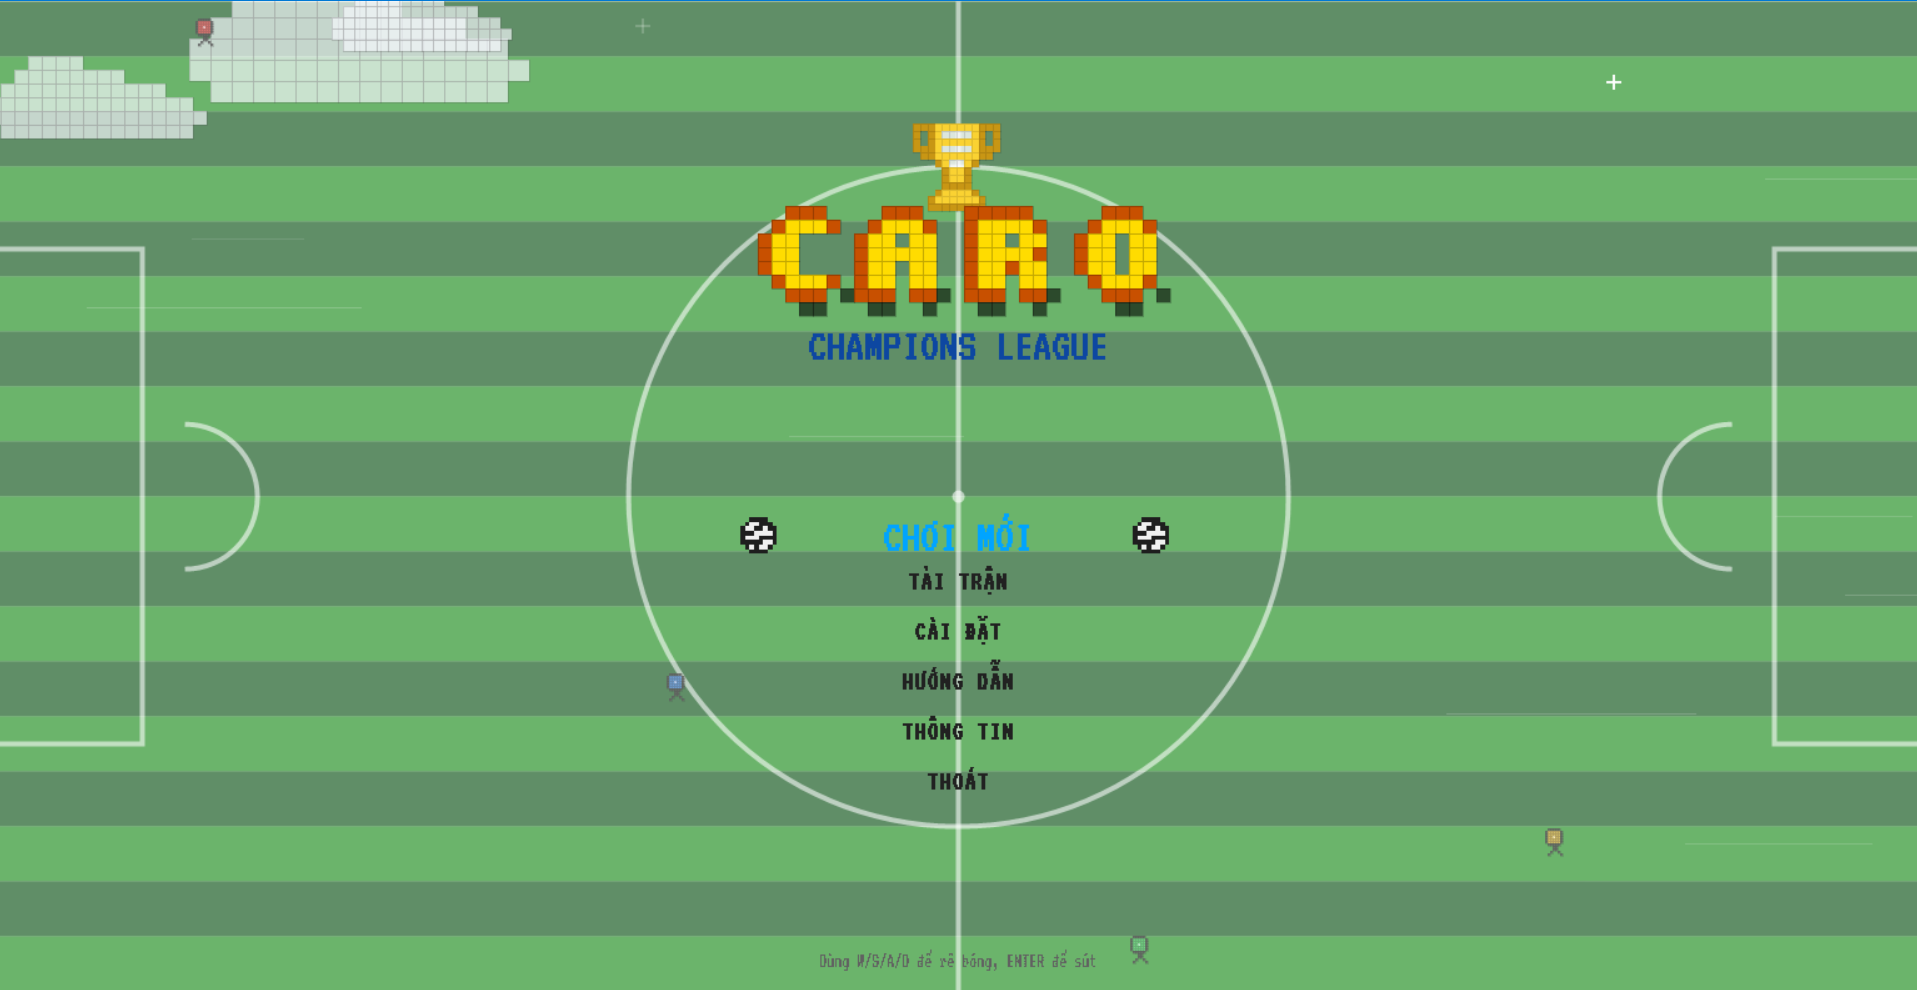
\includegraphics[width=0.9\linewidth]{images/ch4_menu.png}
\end{table}

\captionsetup{type=lstlisting}
\renewcommand{\arraystretch}{0.8}
\captionof{lstlisting}{Mã nguồn RenderMenuScreen và bố cục tiêu đề}\label{lst:ch4_menu_render}
\begin{longtable}{|>{\ttfamily\small\color{black}\raggedleft\arraybackslash}p{0.8cm}|>{\ttfamily\small\color{black}\arraybackslash}p{0.85\linewidth}|}
\hline
\normalfont\bfseries STT & \normalfont\bfseries Mã nguồn \\ \hline
1 & \cppkw{void} RenderMenuScreen(\cpptype{HDC} hdc, \cppkw{int} selectedOption, \cppkw{int} screenWidth, \cppkw{int} screenHeight) \\ \hline
2 & \{ \\ \hline
3 & \ \ Gdiplus::Graphics g(hdc); \\ \hline
4 & \ \ DrawProceduralStadium(g, screenWidth, screenHeight, true); \\ \hline
5 & \ \ Gdiplus::SolidBrush lightGlassBrush(Gdiplus::Color(80, 255, 255, 255)); \\ \hline
6 & \ \ g.FillRectangle(\&lightGlassBrush, 0, 0, screenWidth, screenHeight); \\ \hline
7 &  \\ \hline
8 & \ \ \cppkw{int} cupYOffset = UIScaler::SY((\cppkw{int})(sin(g\_GlobalAnimTime * 2.5f) * 10.0f)); \\ \hline
9 & \ \ DrawPixelTrophy(g, screenWidth / 2, screenHeight / 4 - UIScaler::SY(85) + cupYOffset, UIScaler::S(100)); \\ \hline
10 &  \\ \hline
11 & \ \ \cppkw{static} \cpptype{PixelModel} titleModel; \\ \hline
12 & \ \ \cppkw{static} std::map<int, Gdiplus::Color> titlePalette; \\ \hline
13 & \ \ \cppkw{if} (!titleModel.isLoaded) \{ \\ \hline
14 & \ \ \ \ titleModel = LoadPixelModel("Asset/models/bg/title\_caro.txt"); \\ \hline
15 & \ \ \ \ titlePalette[1] = ToGdiColor(Theme::TitleBorder); \\ \hline
16 & \ \ \ \ titlePalette[2] = ToGdiColor(Theme::TitleFill); \\ \hline
17 & \ \ \ \ titlePalette[3] = ToGdiColor(Theme::TitleShadow); \} \\ \hline
18 & \ \ DrawPixelModel(g, titleModel, screenWidth / 2, screenHeight / 4 + UIScaler::SY(20), UIScaler::S(500), titlePalette); \\ \hline
19 & \} \\ \hline
\end{longtable}

\subsection*{4.6.2. PlayScreen}
\addcontentsline{toc}{subsection}{\textcolor{black}{4.6.2. PlayScreen}}

\setlength{\parindent}{1.5em} PlayScreen tập trung vào tính rõ ràng và phản hồi thị giác:
\begin{itemize}
  \item Lưới cờ vẽ bằng GDI để giữ sắc nét.
  \item Cursor neon đổi màu theo lượt (cam cho P1, cyan cho P2).
  \item Highlight nước đi cuối và chuỗi thắng với hiệu ứng pulse.
  \item Animation cầu thủ sử dụng \texttt{DrawPixelAction} (idle/run/win/sad).
\end{itemize}
\setlength{\parindent}{1.5em} Phần logic cập nhật thời gian và trạng thái cũng làm nền cho UI (đếm giờ, thông báo thắng).

\setlength{\parindent}{1.5em} Trên PlayScreen, các chuỗi hiển thị như \texttt{play\_format} và \texttt{play\_turn} được lấy qua \texttt{GetText} nhằm đảm bảo đa ngôn ngữ. Việc dựng text score theo \texttt{state->targetScore} và \texttt{state->isP1Turn} giúp UI luôn đồng bộ với PlayState.

\setlength{\parindent}{1.5em} Bố cục gồm hai tab trái/phải cho thông tin người chơi, ở giữa là bàn cờ. Kích thước bàn cờ được tính động theo vùng trống (min giữa chiều rộng và chiều cao trừ biên), sau đó quy đổi thành \texttt{cellSize}. Trên cùng là scoreboard và đồng hồ đếm thời gian dạng ``glass panel'' có viền phát sáng theo lượt.

\begin{table}[H]
\caption*{Hình 4.4: Hình minh họa PlayScreen}
\addcontentsline{lof}{figure}{Hình 4.4: Hình minh họa PlayScreen}
\centering
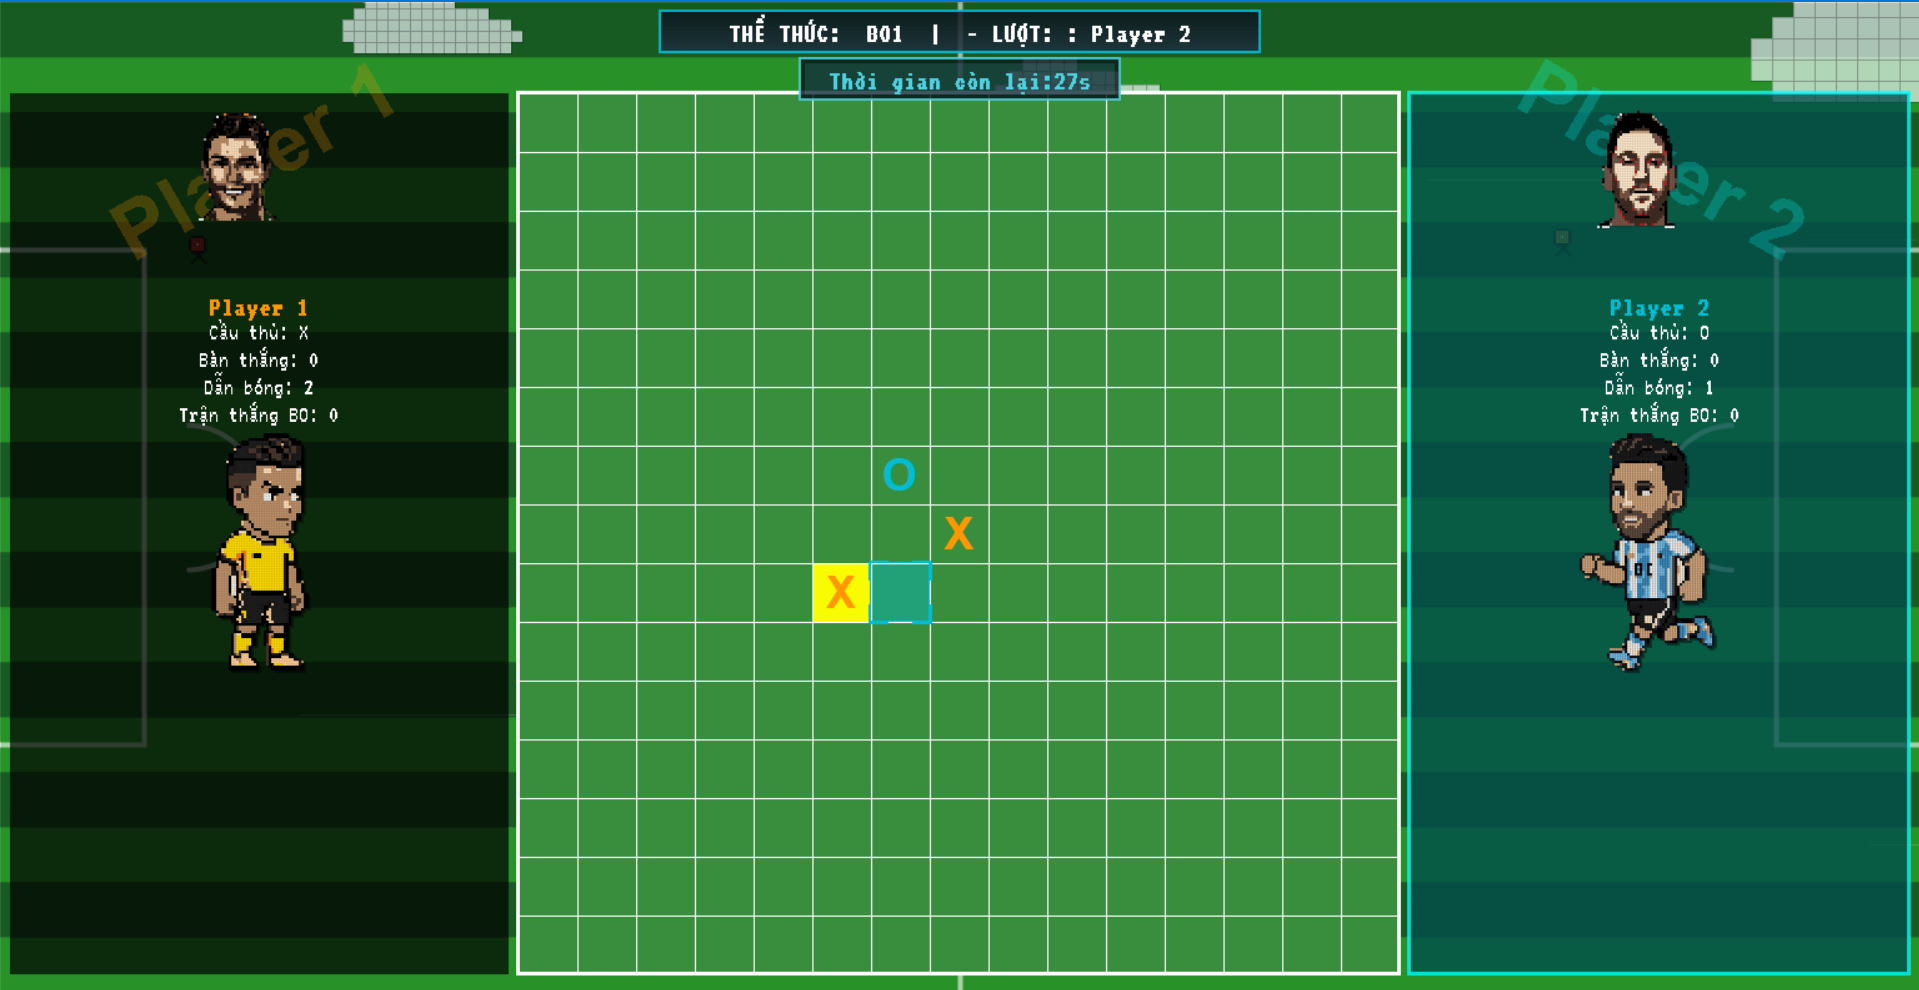
\includegraphics[width=0.9\linewidth]{images/ch4_play.png}
\end{table}

\captionsetup{type=lstlisting}
\renewcommand{\arraystretch}{0.8}
\captionof{lstlisting}{Mã nguồn RenderPlayScreen: tính kích thước và vẽ bàn cờ}\label{lst:ch4_play_render}
\begin{longtable}{|>{\ttfamily\small\color{black}\raggedleft\arraybackslash}p{0.8cm}|>{\ttfamily\small\color{black}\arraybackslash}p{0.85\linewidth}|}
\hline
\normalfont\bfseries STT & \normalfont\bfseries Mã nguồn \\ \hline
1 & \cppkw{void} RenderPlayScreen(\cpptype{HDC} hdc, \cppkw{const} \cpptype{PlayState} *state, \cppkw{int} screenWidth, \cppkw{int} screenHeight, \cppkw{const} \cpptype{GameConfig} *config) \\ \hline
2 & \{ \\ \hline
3 & \ \ Gdiplus::Graphics g(hdc); \\ \hline
4 & \ \ DrawProceduralStadium(g, screenWidth, screenHeight); \\ \hline
5 &  \\ \hline
6 & \ \ \cppkw{int} availableHeight = screenHeight - UIScaler::SY(120); \\ \hline
7 & \ \ \cppkw{int} availableWidth = screenWidth - UIScaler::SX(300); \\ \hline
8 & \ \ \cppkw{int} maxBoardSize = availableWidth < availableHeight ? availableWidth : availableHeight; \\ \hline
9 & \ \ \cppkw{int} dynamicCellSize = maxBoardSize / state->boardSize; \\ \hline
10 & \ \ \cppkw{int} boardPixelSize = state->boardSize * dynamicCellSize; \\ \hline
11 & \ \ \cppkw{int} startX = (screenWidth - boardPixelSize) / 2; \\ \hline
12 & \ \ \cppkw{int} startY = (screenHeight - boardPixelSize) / 2 + UIScaler::SY(40); \\ \hline
13 &  \\ \hline
14 & \ \ DrawGameBoard(g, hdc, state, dynamicCellSize, startX, startY); \\ \hline
15 &  \\ \hline
16 & \ \ \cppkw{int} scoreW = UIScaler::SX(600); \\ \hline
17 & \ \ \cppkw{int} scoreH = UIScaler::SY(45); \\ \hline
18 & \ \ \cppkw{int} scoreX = (screenWidth - scoreW) / 2; \\ \hline
19 & \ \ \cppkw{int} scoreY = UIScaler::SY(10); \\ \hline
20 & \ \ std::wstring formatText = GetText("play\_format") + L" BO" + std::to\_wstring(state->targetScore); \\ \hline
21 & \ \ std::wstring turnText = GetText("play\_turn") + L": " + (state->isP1Turn ? state->p1.name : state->p2.name); \\ \hline
22 & \ \ std::wstring fullScoreText = formatText + L"  |  " + turnText; \\ \hline
23 & \ \ COLORREF turnColor = state->isP1Turn ? ToCOLORREF(Palette::OrangeNormal) : ToCOLORREF(Palette::CyanNormal); \\ \hline
24 & \ \ \cppkw{float} pulseScore = 0.6f + sin(g\_GlobalAnimTime * 6.0f) * 0.4f; \\ \hline
25 & \ \ BYTE scoreAlpha = (BYTE)(130 + pulseScore * 125); \\ \hline
26 & \ \ Gdiplus::LinearGradientBrush scoreBg(Gdiplus::Point(scoreX, scoreY), Gdiplus::Point(scoreX, scoreY + scoreH), Gdiplus::Color(210, 10, 15, 25), Gdiplus::Color(210, 30, 45, 65)); \\ \hline
27 & \ \ g.FillRectangle(\&scoreBg, scoreX, scoreY, scoreW, scoreH); \\ \hline
28 & \ \ Gdiplus::Pen scoreBorder(Gdiplus::Color(scoreAlpha, GetRValue(turnColor), GetGValue(turnColor), GetBValue(turnColor)), 2.5f); \\ \hline
29 & \ \ g.DrawRectangle(\&scoreBorder, scoreX, scoreY, scoreW, scoreH); \\ \hline
30 & \} \\ \hline
\end{longtable}

\subsection*{4.6.3. Pause Game}
\addcontentsline{toc}{subsection}{\textcolor{black}{4.6.3. Pause Game}}

\setlength{\parindent}{1.5em} Pause menu là lớp phủ trực tiếp lên gameplay, nhằm giữ ngữ cảnh trong khi vẫn giảm độ tập trung vào bàn cờ. Màn hình gồm hai khối chính: khung menu bên trái và cột hướng dẫn điều khiển bên phải. Các mục như Resume, BGM, Volume, Save, Exit được trình bày theo danh sách dọc, trong đó volume có thanh trượt trực quan.

\setlength{\parindent}{1.5em} Lớp overlay dùng \texttt{Theme::GlassWhite} để giảm độ tương phản nền, tạo hiệu ứng "mờ" nhưng không làm mất hoàn toàn bối cảnh game. Điều này giúp người chơi vẫn nhận biết trạng thái ván đang tạm dừng.

\setlength{\parindent}{1.5em} Khi tạm dừng, hệ thống dùng nền kính trắng mờ để giảm nhiễu thị giác; banner ``Pause'' và icon còi (whistle) được vẽ bằng pixel art để giữ đồng nhất phong cách.

\begin{table}[H]
\caption*{Hình 4.5: Hình minh họa Pause Game}
\addcontentsline{lof}{figure}{Hình 4.5: Hình minh họa Pause Game}
\centering
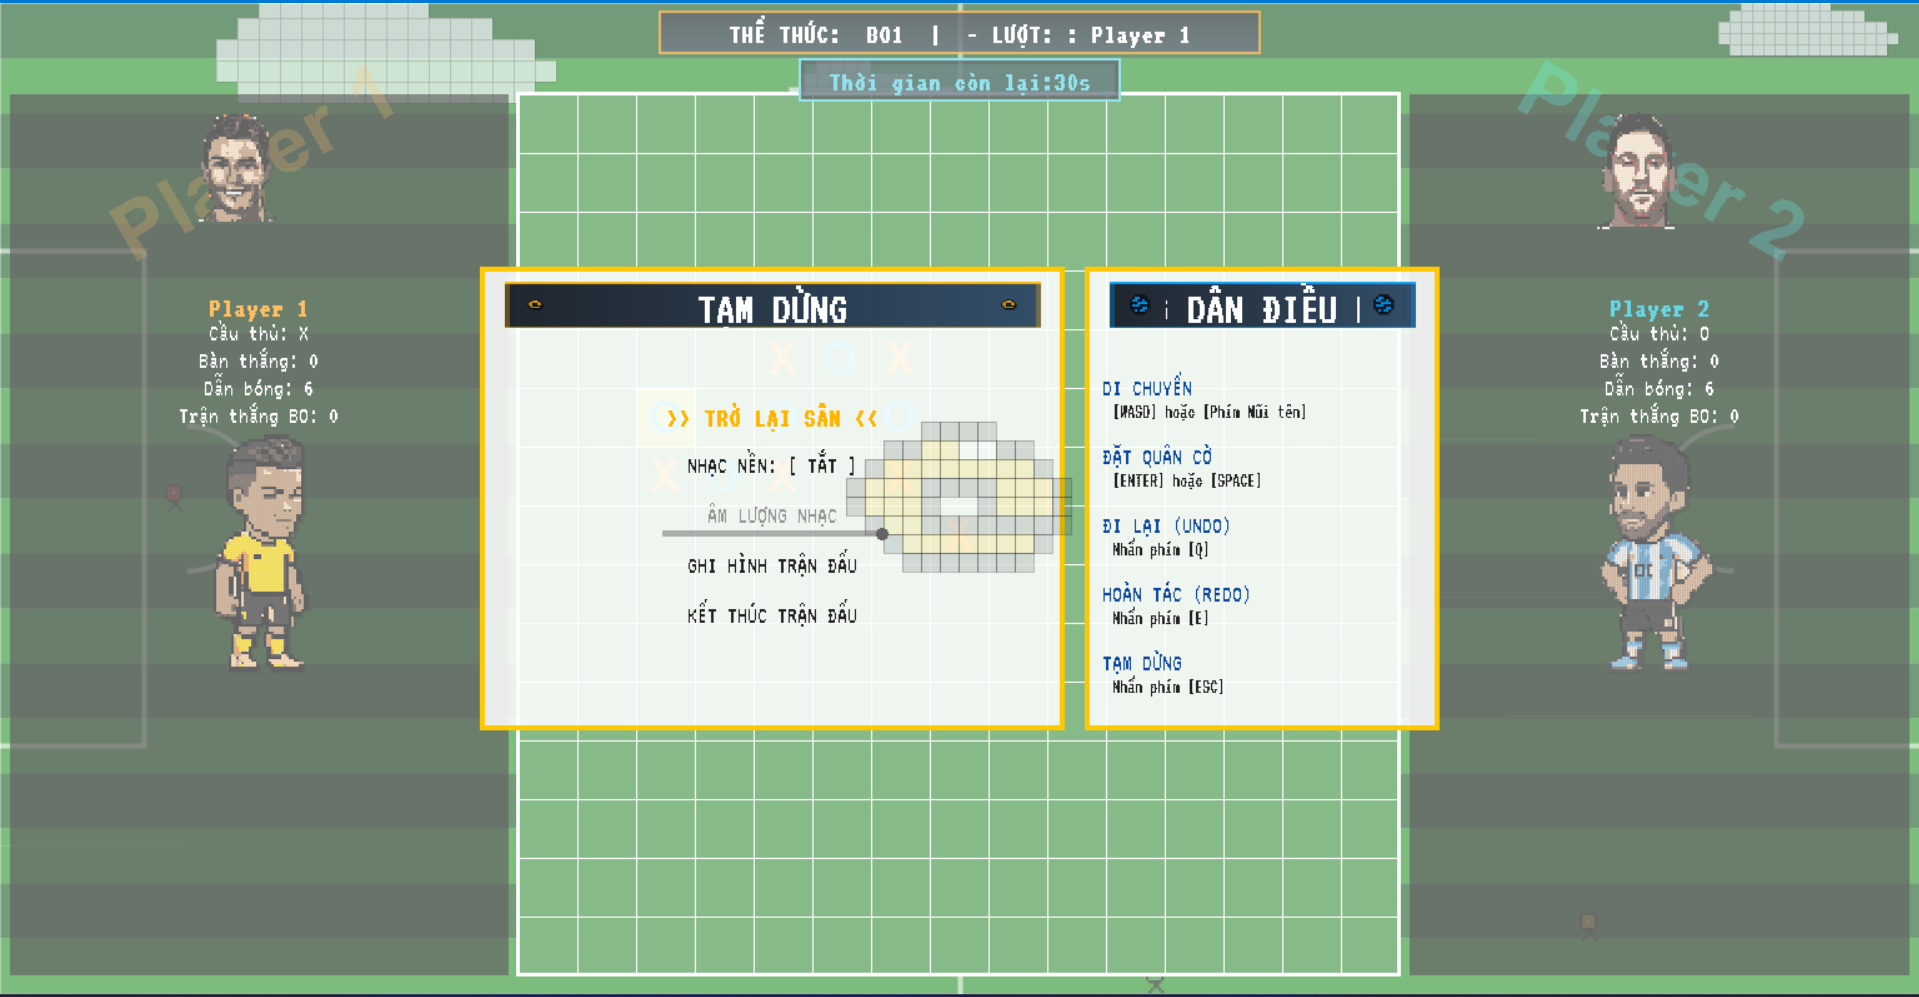
\includegraphics[width=0.9\linewidth]{images/ch4_pause.png}
\end{table}

\captionsetup{type=lstlisting}
\renewcommand{\arraystretch}{0.8}
\captionof{lstlisting}{Mã nguồn Lớp phủ Pause Menu trong RenderPlayScreen}\label{lst:ch4_pause_render}
\begin{longtable}{|>{\ttfamily\small\color{black}\raggedleft\arraybackslash}p{0.8cm}|>{\ttfamily\small\color{black}\arraybackslash}p{0.85\linewidth}|}
\hline
\normalfont\bfseries STT & \normalfont\bfseries Mã nguồn \\ \hline
1 & \cppkw{if} (state->status == MATCH\_PAUSED) \\ \hline
2 & \{ \\ \hline
3 & \ \ \cpptype{Gdiplus::SolidBrush} shadowBrush2(Gdiplus::Color(100, 255, 255, 255)); \\ \hline
4 & \ \ g.FillRectangle(\&shadowBrush2, 0, 0, screenWidth, screenHeight); \\ \hline
5 &  \\ \hline
6 & \ \ \cppkw{int} menuW = UIScaler::SX(580), menuH = UIScaler::SY(500); \\ \hline
7 & \ \ \cppkw{int} guideW = UIScaler::SX(350); \\ \hline
8 & \ \ \cppkw{int} gap = UIScaler::SX(25); \\ \hline
9 & \ \ \cppkw{int} totalW = (g\_CurrentSubMenu == SUB\_MAIN) ? (menuW + gap + guideW) : menuW; \\ \hline
10 & \ \ \cppkw{int} totalStartX = (screenWidth - totalW) / 2; \\ \hline
11 &  \\ \hline
12 & \ \ \cppkw{int} menuX = totalStartX; \\ \hline
13 & \ \ \cppkw{int} menuY = (screenHeight - menuH) / 2; \\ \hline
14 & \ \ \cpptype{Gdiplus::SolidBrush} bgBrush(ToGdiColor(Theme::GlassWhite)); \\ \hline
15 & \ \ g.FillRectangle(\&bgBrush, menuX, menuY, menuW, menuH); \\ \hline
16 & \ \ \cpptype{Gdiplus::Pen} yellowBorder(ToGdiColor(Theme::PanelYellowBorder), 4.0f); \\ \hline
17 & \ \ g.DrawRectangle(\&yellowBorder, menuX, menuY, menuW, menuH); \\ \hline
18 & \ \ DrawPixelBanner(g, hdc, GetText("pause\_title").c\_str(), menuX + menuW / 2, menuY + UIScaler::SY(40), menuW - UIScaler::SX(20), ToCOLORREF(Palette::White), RGB(255, 180, 0), "Asset/models/bg/whistle.txt"); \\ \hline
19 & \} \\ \hline
\end{longtable}

\subsection*{4.6.4. MatchConfigScreen}
\addcontentsline{toc}{subsection}{\textcolor{black}{4.6.4. MatchConfigScreen}}

\setlength{\parindent}{1.5em} Màn hình cấu hình trận đấu có hai trang, áp dụng UI điều hướng rõ ràng:
\begin{itemize}
  \item Trang 1: cấu hình chế độ, PvP/PvE, độ khó, thời gian, số ván.
  \item Trang 2: cấu hình avatar và tên người chơi với input trực tiếp.
\end{itemize}
\setlength{\parindent}{1.5em} Màu sắc và font thay đổi theo lựa chọn để nhấn mạnh mục đang focus; mỗi giá trị được hiển thị trong khung riêng, tạo cảm giác ``form'' rõ ràng.

\setlength{\parindent}{1.5em} Layout chính là một panel kính giữa màn hình, chia hai cột (nhãn và giá trị). Ở trang 2, mỗi người chơi là một ``card'' riêng với avatar, tên, và hiệu ứng glow khi đang được chọn.

\begin{table}[H]
\caption*{Hình 4.6: Hình minh họa MatchConfigScreen - trang 1}
\addcontentsline{lof}{figure}{Hình 4.6: Hình minh họa MatchConfigScreen - trang 1}
\centering
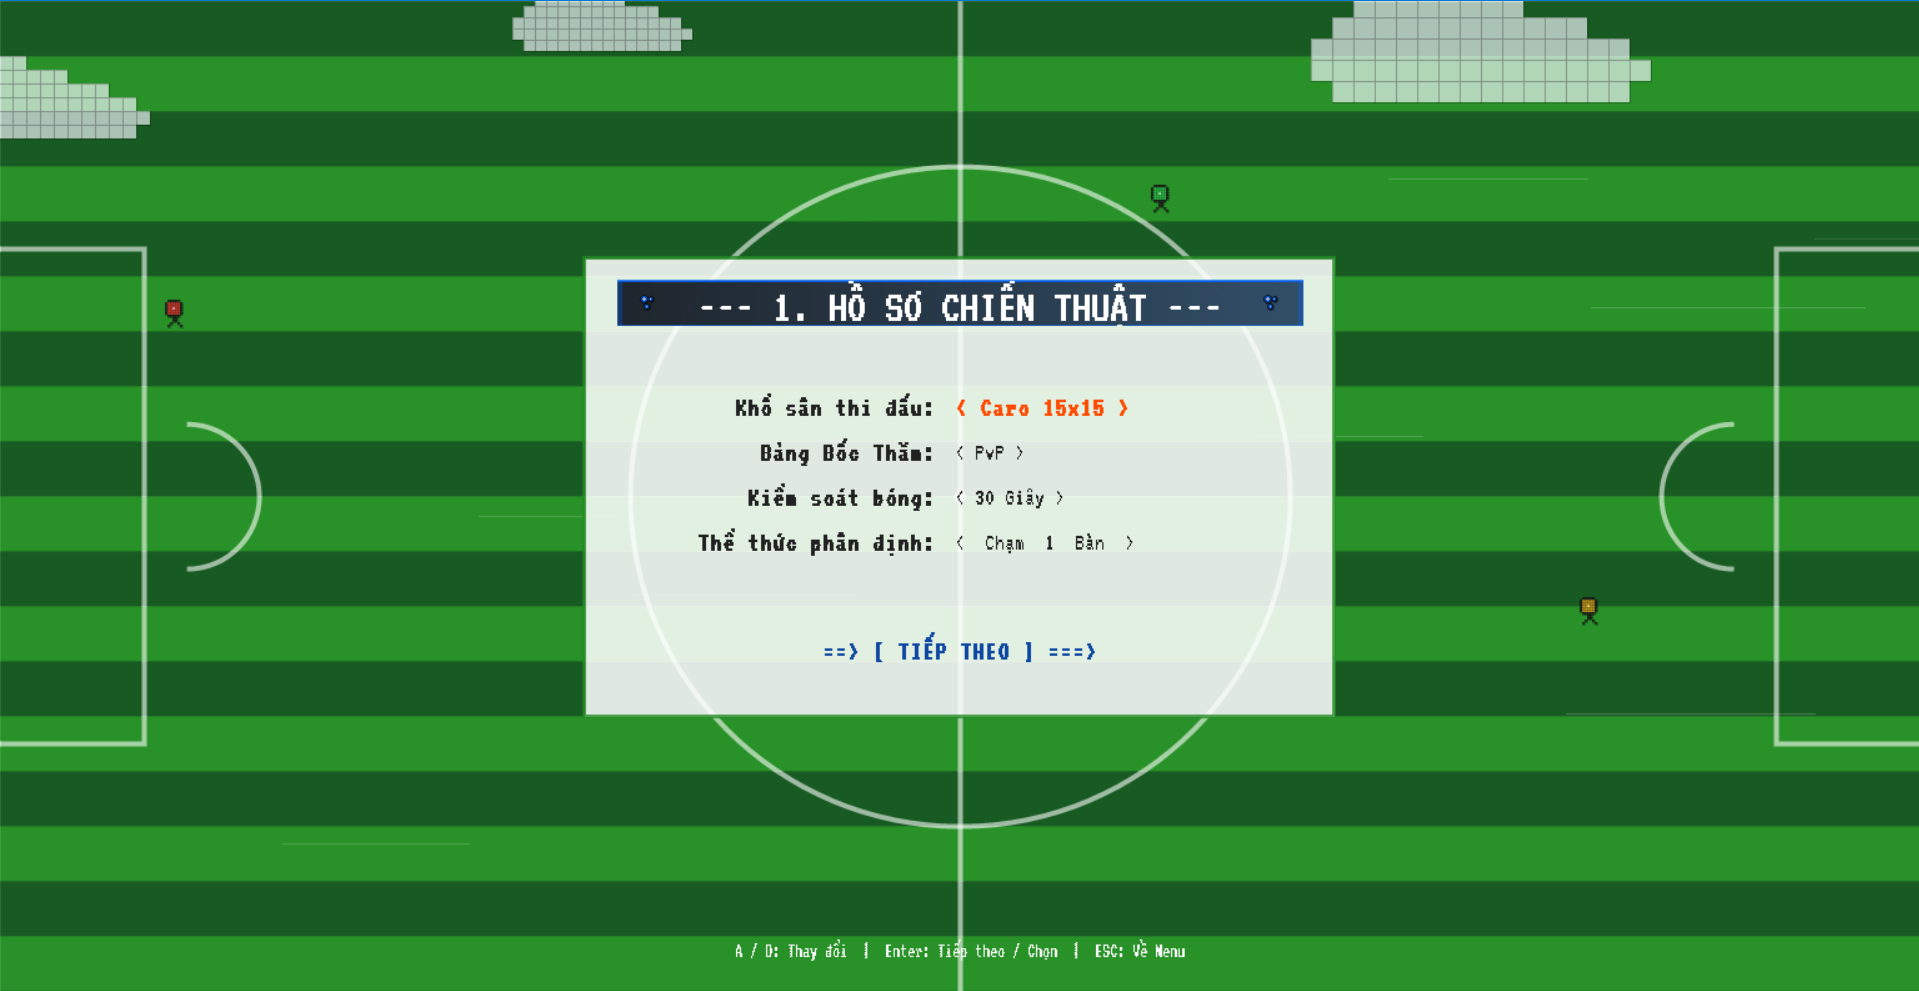
\includegraphics[width=0.9\linewidth]{images/ch4_match_config.png}
\end{table}

\begin{table}[H]
\caption*{Hình 4.7: Hình minh họa MatchConfigScreen - trang 2}
\addcontentsline{lof}{figure}{Hình 4.7: Hình minh họa MatchConfigScreen - trang 2}
\centering
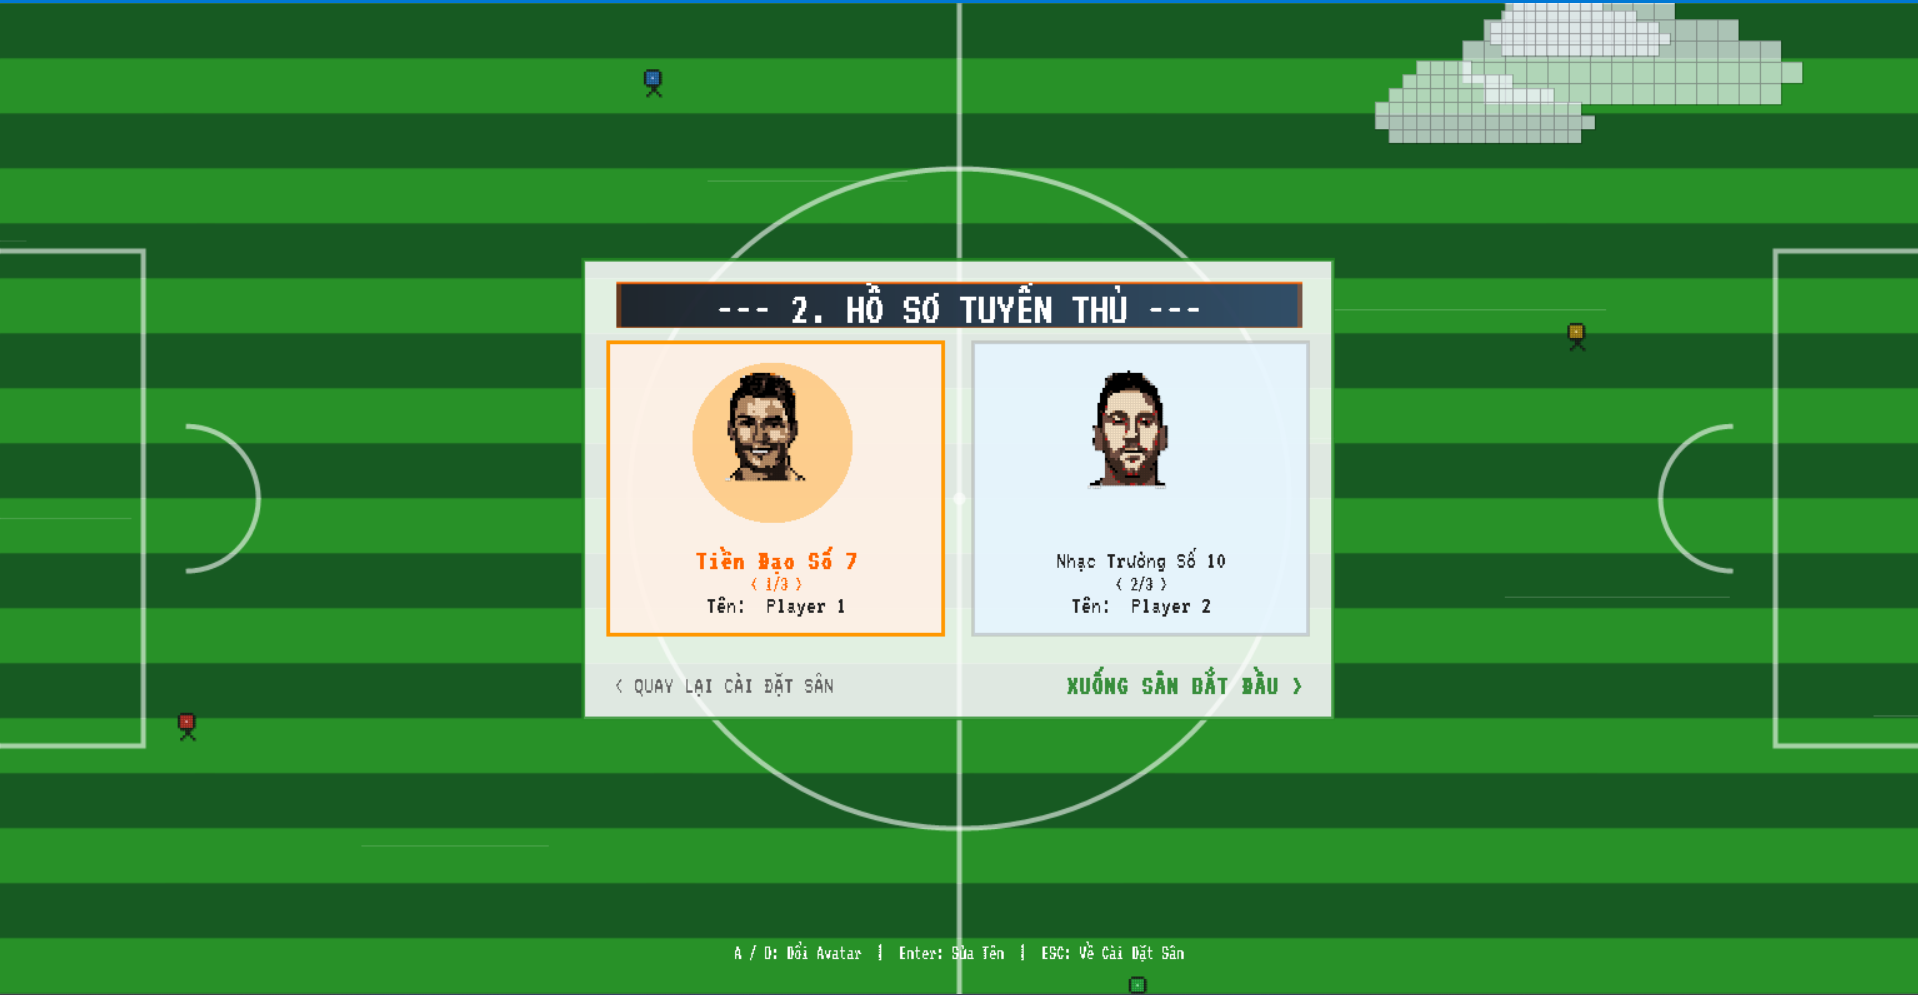
\includegraphics[width=0.9\linewidth]{images/ch4_match_config_2.png}
\end{table}

\captionsetup{type=lstlisting}
\renewcommand{\arraystretch}{0.8}
\captionof{lstlisting}{Mã nguồn RenderMatchConfigScreen: panel và banner}\label{lst:ch4_match_config_render}
\begin{longtable}{|>{\ttfamily\small\color{black}\raggedleft\arraybackslash}p{0.8cm}|>{\ttfamily\small\color{black}\arraybackslash}p{0.85\linewidth}|}
\hline
\normalfont\bfseries STT & \normalfont\bfseries Mã nguồn \\ \hline
1 & \cppkw{void} RenderMatchConfigScreen(\cpptype{HDC} hdc, \cppkw{int} selectedOption, \cppkw{const} \cpptype{PlayState} *config, \cppkw{int} screenWidth, \cppkw{int} screenHeight) \\ \hline
2 & \{ \\ \hline
3 & \ \ Gdiplus::Graphics g(hdc); \\ \hline
4 & \ \ DrawProceduralStadium(g, screenWidth, screenHeight); \\ \hline
5 &  \\ \hline
6 & \ \ Gdiplus::SolidBrush whitePanel(ToGdiColor(Theme::GlassWhite)); \\ \hline
7 & \ \ \cppkw{int} panelW = UIScaler::SX(750); \\ \hline
8 & \ \ \cppkw{int} panelH = UIScaler::SY(500); \\ \hline
9 & \ \ \cppkw{int} panelX = (screenWidth - panelW) / 2; \\ \hline
10 & \ \ \cppkw{int} panelY = (screenHeight - panelH) / 2 - UIScaler::SY(10); \\ \hline
11 & \ \ g.FillRectangle(\&whitePanel, panelX, panelY, panelW, panelH); \\ \hline
12 & \ \ Gdiplus::Pen panelPen(ToGdiColor(Theme::PanelGreenBorder), 3.0f); \\ \hline
13 & \ \ g.DrawRectangle(\&panelPen, panelX, panelY, panelW, panelH); \\ \hline
14 & \ \ DrawPixelBanner(g, hdc, GetText("config\_page1").c\_str(), screenWidth / 2, panelY + UIScaler::SY(50), panelW - UIScaler::SX(40), ToCOLORREF(Palette::White), RGB(0, 100, 255), "Asset/models/bg/gears.txt"); \\ \hline
15 & \} \\ \hline
\end{longtable}

\subsection*{4.6.5. SettingScreen}
\addcontentsline{toc}{subsection}{\textcolor{black}{4.6.5. SettingScreen}}

\setlength{\parindent}{1.5em} SettingScreen là ví dụ điển hình của layout dạng bảng và thanh trượt:
\begin{itemize}
  \item Panel kính trắng, viền màu xanh.
  \item Banner tiêu đề có icon bánh răng.
  \item Thanh volume vẽ bằng GDI+, có bar track, fill, thumb.
  \item Mục bị disable sẽ đổi màu xám để giảm độ nổi bật.
\end{itemize}
\setlength{\parindent}{1.5em} Các mục bật/tắt được trình bày dưới dạng nhãn trạng thái, trong khi thanh trượt thể hiện mức âm lượng bằng tỉ lệ chiều dài.

\setlength{\parindent}{1.5em} Hệ thống chia panel thành hai cột: nhãn (trái) và giá trị (phải). Thanh trượt âm lượng dùng GDI+ để vẽ nền, phần fill và thumb, đồng thời đổi màu khi mục đang được chọn.

\setlength{\parindent}{1.5em} Các màu của thanh trượt lấy từ \texttt{Theme::BarTrack}, \texttt{Theme::BarFillSelected} và \texttt{Theme::BarFillNormal}, giúp nhất quán với bảng màu tổng thể. Khi tắt BGM/SFX, màu mục chuyển xám để biểu đạt trạng thái disable.

\begin{table}[H]
\caption*{Hình 4.8: Hình minh họa SettingScreen}
\addcontentsline{lof}{figure}{Hình 4.8: Hình minh họa SettingScreen}
\centering
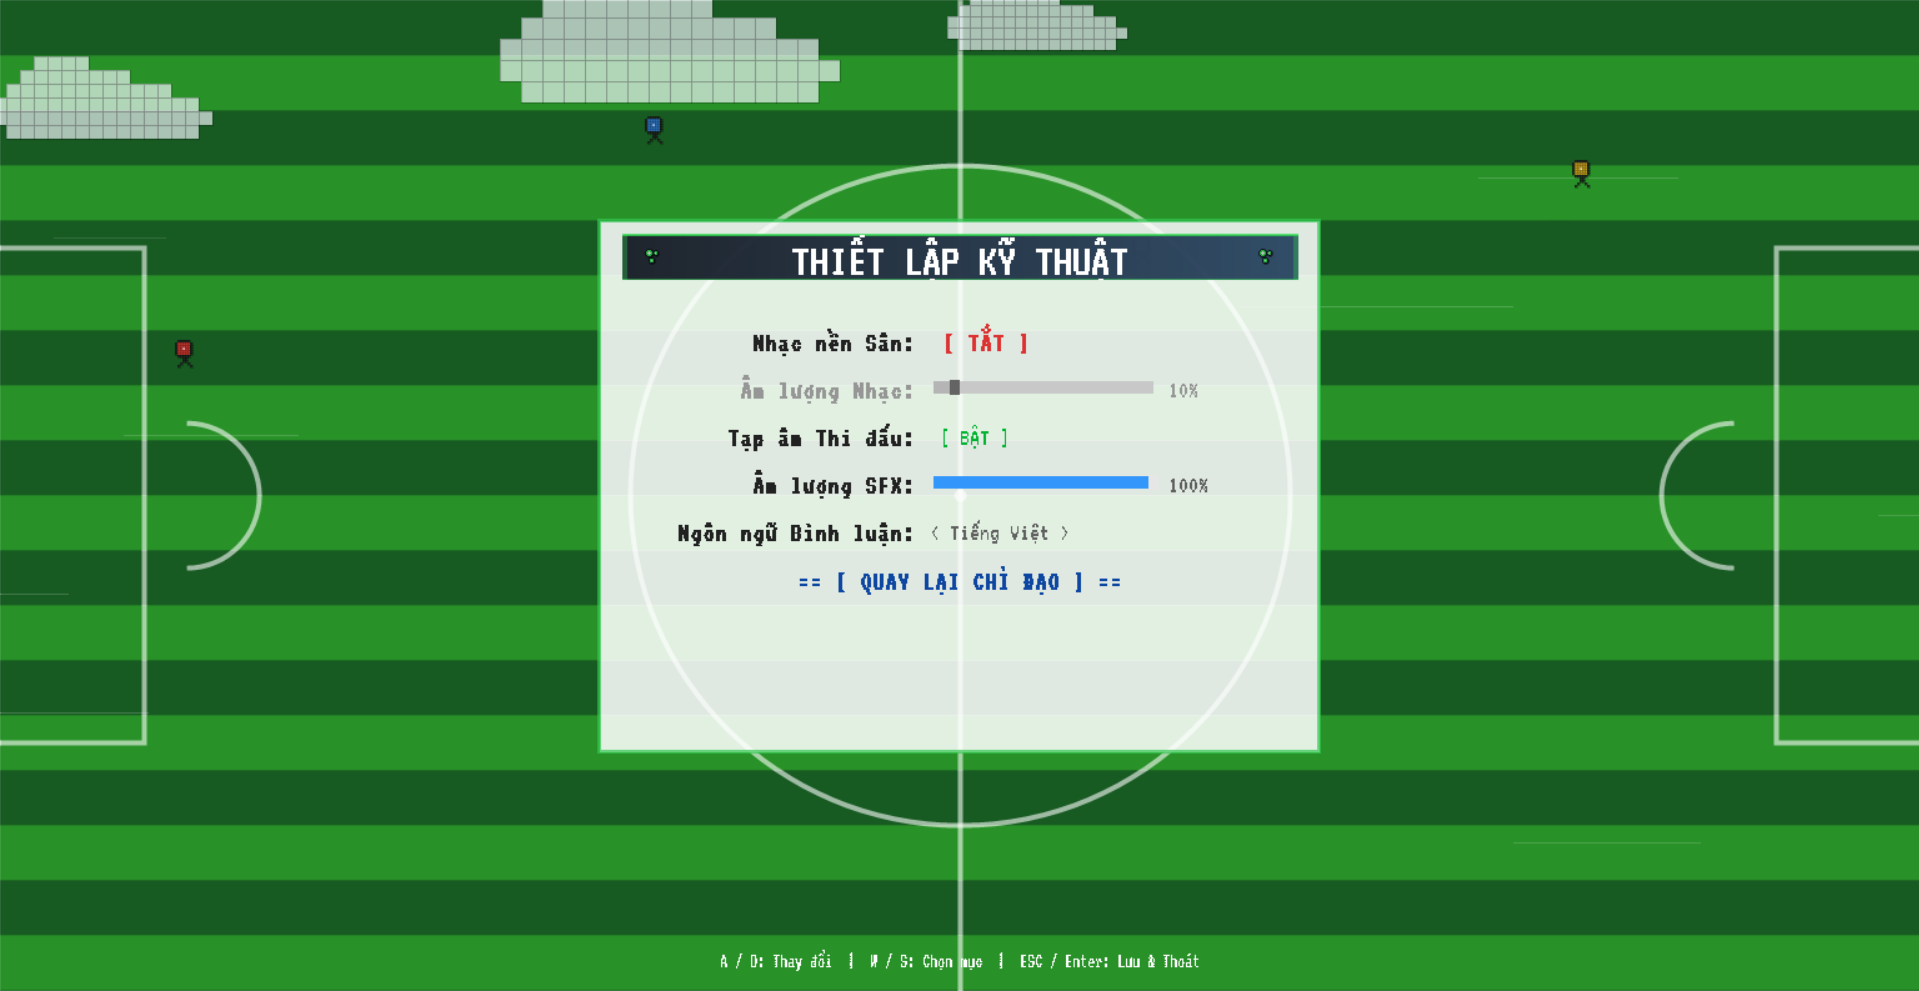
\includegraphics[width=0.9\linewidth]{images/ch4_setting.png}
\end{table}

\captionsetup{type=lstlisting}
\renewcommand{\arraystretch}{0.8}
\captionof{lstlisting}{Mã nguồn RenderSettingScreen: panel và thanh volume}\label{lst:ch4_setting_render}
\begin{longtable}{|>{\ttfamily\small\color{black}\raggedleft\arraybackslash}p{0.8cm}|>{\ttfamily\small\color{black}\arraybackslash}p{0.85\linewidth}|}
\hline
\normalfont\bfseries STT & \normalfont\bfseries Mã nguồn \\ \hline
1 & \cppkw{void} RenderSettingScreen(\cpptype{HDC} hdc, \cppkw{const} \cpptype{GameConfig} *config, \cppkw{int} selectedOption, \cppkw{int} screenWidth, \cppkw{int} screenHeight) \\ \hline
2 & \{ \\ \hline
3 & \ \ Gdiplus::Graphics g(hdc); \\ \hline
4 & \ \ DrawProceduralStadium(g, screenWidth, screenHeight); \\ \hline
5 &  \\ \hline
6 & \ \ \cppkw{int} panelW = UIScaler::SX(720); \\ \hline
7 & \ \ \cppkw{int} panelH = UIScaler::SY(580); \\ \hline
8 & \ \ \cppkw{int} panelX = (screenWidth - panelW) / 2; \\ \hline
9 & \ \ \cppkw{int} panelY = (screenHeight - panelH) / 2 - UIScaler::SY(10); \\ \hline
10 & \ \ Gdiplus::SolidBrush whitePanel(ToGdiColor(Theme::GlassWhite)); \\ \hline
11 & \ \ g.FillRectangle(\&whitePanel, panelX, panelY, panelW, panelH); \\ \hline
12 & \ \ DrawPixelBanner(g, hdc, GetText("setting\_title").c\_str(), screenWidth / 2, panelY + UIScaler::SY(40), panelW - UIScaler::SX(20), ToCOLORREF(Palette::White), RGB(50, 220, 80), "Asset/models/bg/gears.txt"); \\ \hline
13 & \} \\ \hline
\end{longtable}

\subsection*{4.6.6. LoadGameScreen}
\addcontentsline{toc}{subsection}{\textcolor{black}{4.6.6. LoadGameScreen}}

\setlength{\parindent}{1.5em} Màn hình load game chia thành ba vùng: danh sách slot, thông tin slot, và hành động. Trạng thái tương tác được quản lý rõ ràng:
\begin{itemize}
  \item \texttt{MODE\_SELECT\_SLOT}: chọn slot ở cột trái.
  \item \texttt{MODE\_SELECT\_ACTION}: chọn hành động (Load/Rename/Delete/Back).
  \item \texttt{MODE\_EDIT\_NAME}: nhập tên slot mới.
\end{itemize}
\setlength{\parindent}{1.5em} Điểm UX quan trọng: nếu slot trống sẽ hiển thị thông báo ngắn, tránh thao tác không cần thiết. Các panel được chia cột bằng layout tính theo \texttt{UIScaler} nên luôn cân đối.

\setlength{\parindent}{1.5em} Màn hình gồm ba cột: danh sách slot, thông tin chi tiết và cột hành động/đổi tên. Trạng thái chọn được tô nền bằng màu trong suốt để phân biệt giữa ``đang chọn slot'' và ``đang chọn hành động''.

\setlength{\parindent}{1.5em} Các màu nhấn cho slot lấy từ \texttt{Theme::SlotSelected} và \texttt{Theme::SlotNormal}, đảm bảo đồng bộ với palette chung. Đây là chi tiết nhỏ nhưng giúp UI không bị "lạc tông" giữa các màn hình.

\begin{table}[H]
\caption*{Hình 4.9: Hình minh họa LoadGameScreen}
\addcontentsline{lof}{figure}{Hình 4.9: Hình minh họa LoadGameScreen}
\centering
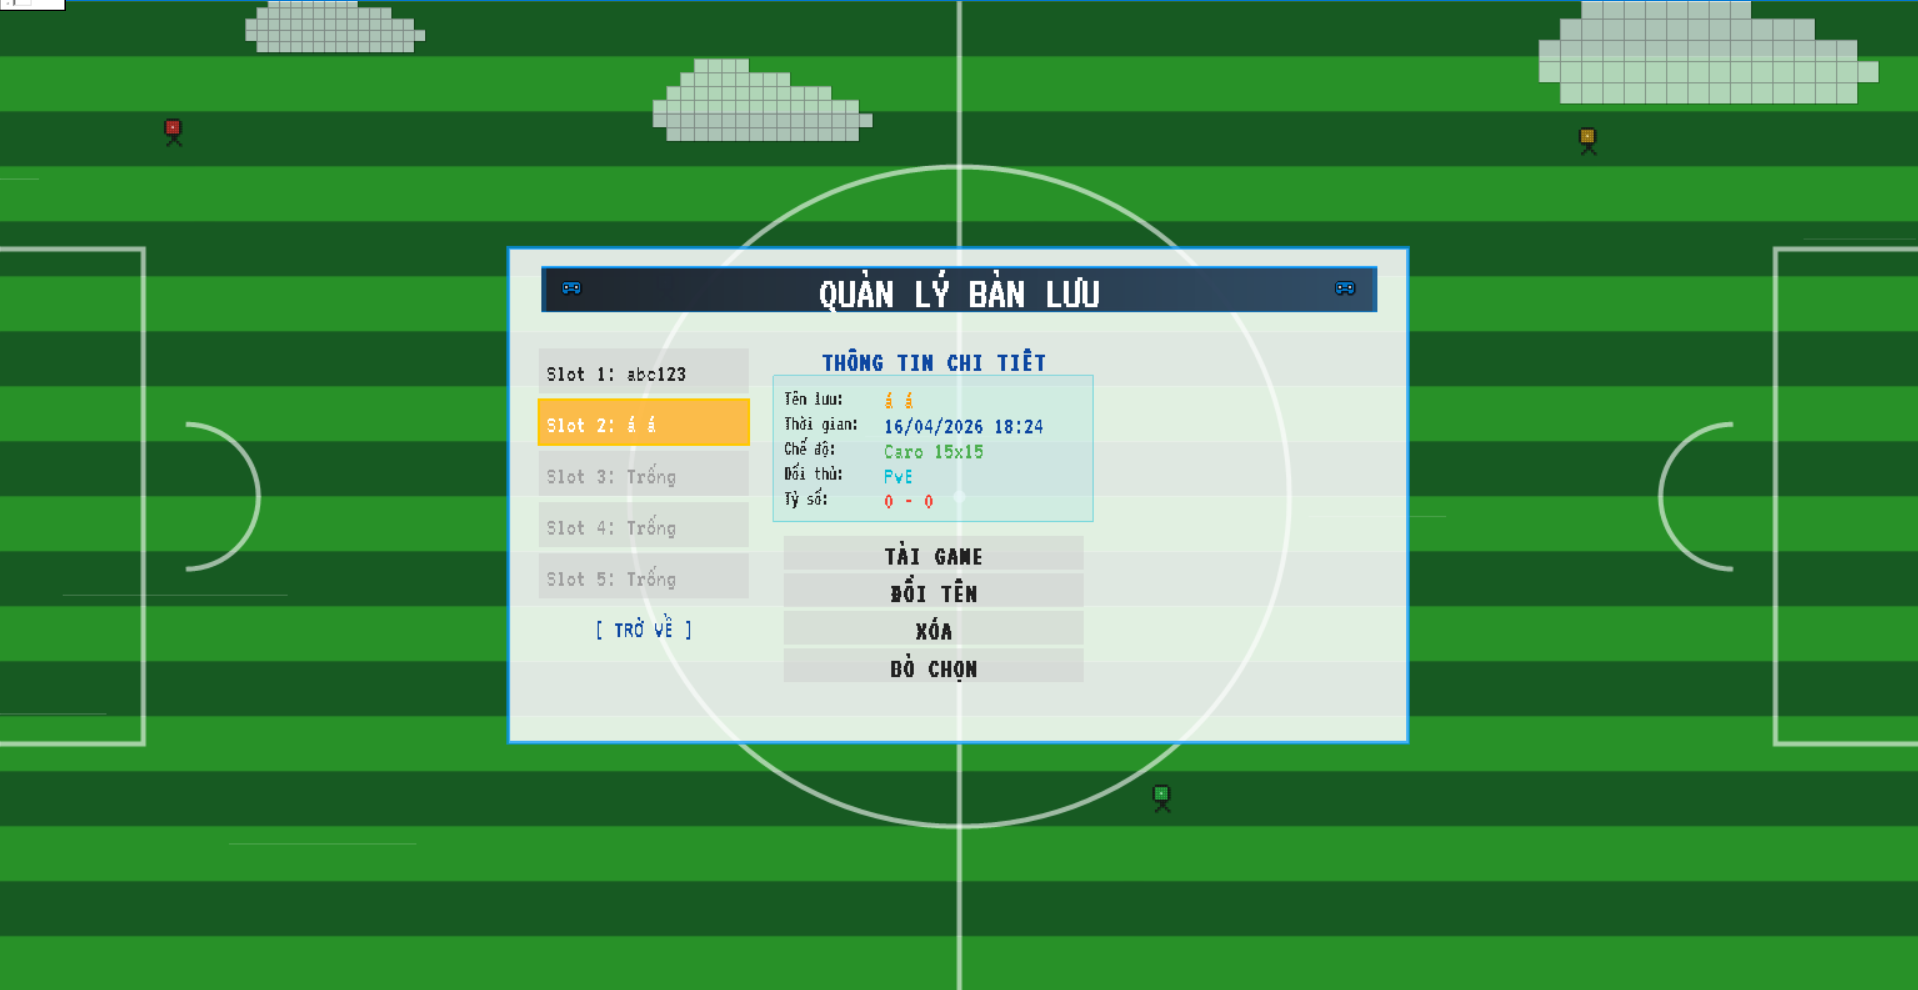
\includegraphics[width=0.9\linewidth]{images/ch4_load_game.png}
\end{table}

\captionsetup{type=lstlisting}
\renewcommand{\arraystretch}{0.8}
\captionof{lstlisting}{Mã nguồn Che do tuong tac va RenderLoadGameScreen}\label{lst:ch4_load_render}
\begin{longtable}{|>{\ttfamily\small\color{black}\raggedleft\arraybackslash}p{0.8cm}|>{\ttfamily\small\color{black}\arraybackslash}p{0.85\linewidth}|}
\hline
\normalfont\bfseries STT & \normalfont\bfseries Mã nguồn \\ \hline
1 & \cppkw{enum} LoadScreenMode \\ \hline
2 & \{ MODE\_SELECT\_SLOT, MODE\_SELECT\_ACTION, MODE\_EDIT\_NAME \}; \\ \hline
3 &  \\ \hline
4 & \cppkw{void} RenderLoadGameScreen(\cpptype{HDC} hdc, \cppkw{int} selectedOption, \cppkw{const} \cpptype{std::wstring} \&statusMessage, \cppkw{int} screenWidth, \cppkw{int} screenHeight) \\ \hline
5 & \{ \\ \hline
6 & \ \ Gdiplus::Graphics g(hdc); \\ \hline
7 & \ \ DrawProceduralStadium(g, screenWidth, screenHeight); \\ \hline
8 &  \\ \hline
9 & \ \ \cppkw{int} panelW = UIScaler::SX(900); \\ \hline
10 & \ \ \cppkw{int} panelH = UIScaler::SY(540); \\ \hline
11 & \ \ \cppkw{int} panelX = (screenWidth - panelW) / 2; \\ \hline
12 & \ \ \cppkw{int} panelY = (screenHeight - panelH) / 2; \\ \hline
13 & \ \ Gdiplus::SolidBrush bgBrush(ToGdiColor(Theme::GlassWhite)); \\ \hline
14 & \ \ g.FillRectangle(\&bgBrush, panelX, panelY, panelW, panelH); \\ \hline
15 & \ \ DrawPixelBanner(g, hdc, GetText("save\_title").c\_str(), screenWidth / 2, panelY + UIScaler::SY(45), panelW - UIScaler::SX(40), ToCOLORREF(Palette::White), RGB(0, 150, 255), "Asset/models/bg/cassette.txt"); \\ \hline
16 & \} \\ \hline
\end{longtable}

\subsection*{4.6.7. AboutScreen}
\addcontentsline{toc}{subsection}{\textcolor{black}{4.6.7. AboutScreen}}

\setlength{\parindent}{1.5em} AboutScreen thể hiện phong cách trình bày thông tin:
\begin{itemize}
  \item Nền sân + lớp kính mờ.
  \item Banner tiêu đề theo ngôn ngữ.
  \item Bảng thành viên với header nền xanh, grid line rõ ràng.
  \item Dòng giảng viên hướng dẫn và công nghệ.
\end{itemize}
\setlength{\parindent}{1.5em} Màu sắc thiên sáng, thể hiện tông sáng nhẹ nhàng hơn so với các màn hình gameplay.

\setlength{\parindent}{1.5em} Bảng thành viên được vẽ như một bảng dữ liệu: có header nền xanh, chia cột, kẻ grid line bằng GDI+ để đảm bảo độ đều. Các dòng chữ căn giữa theo từng cột.

\begin{table}[H]
\caption*{Hình 4.10: Hình minh họa AboutScreen}
\addcontentsline{lof}{figure}{Hình 4.10: Hình minh họa AboutScreen}
\centering
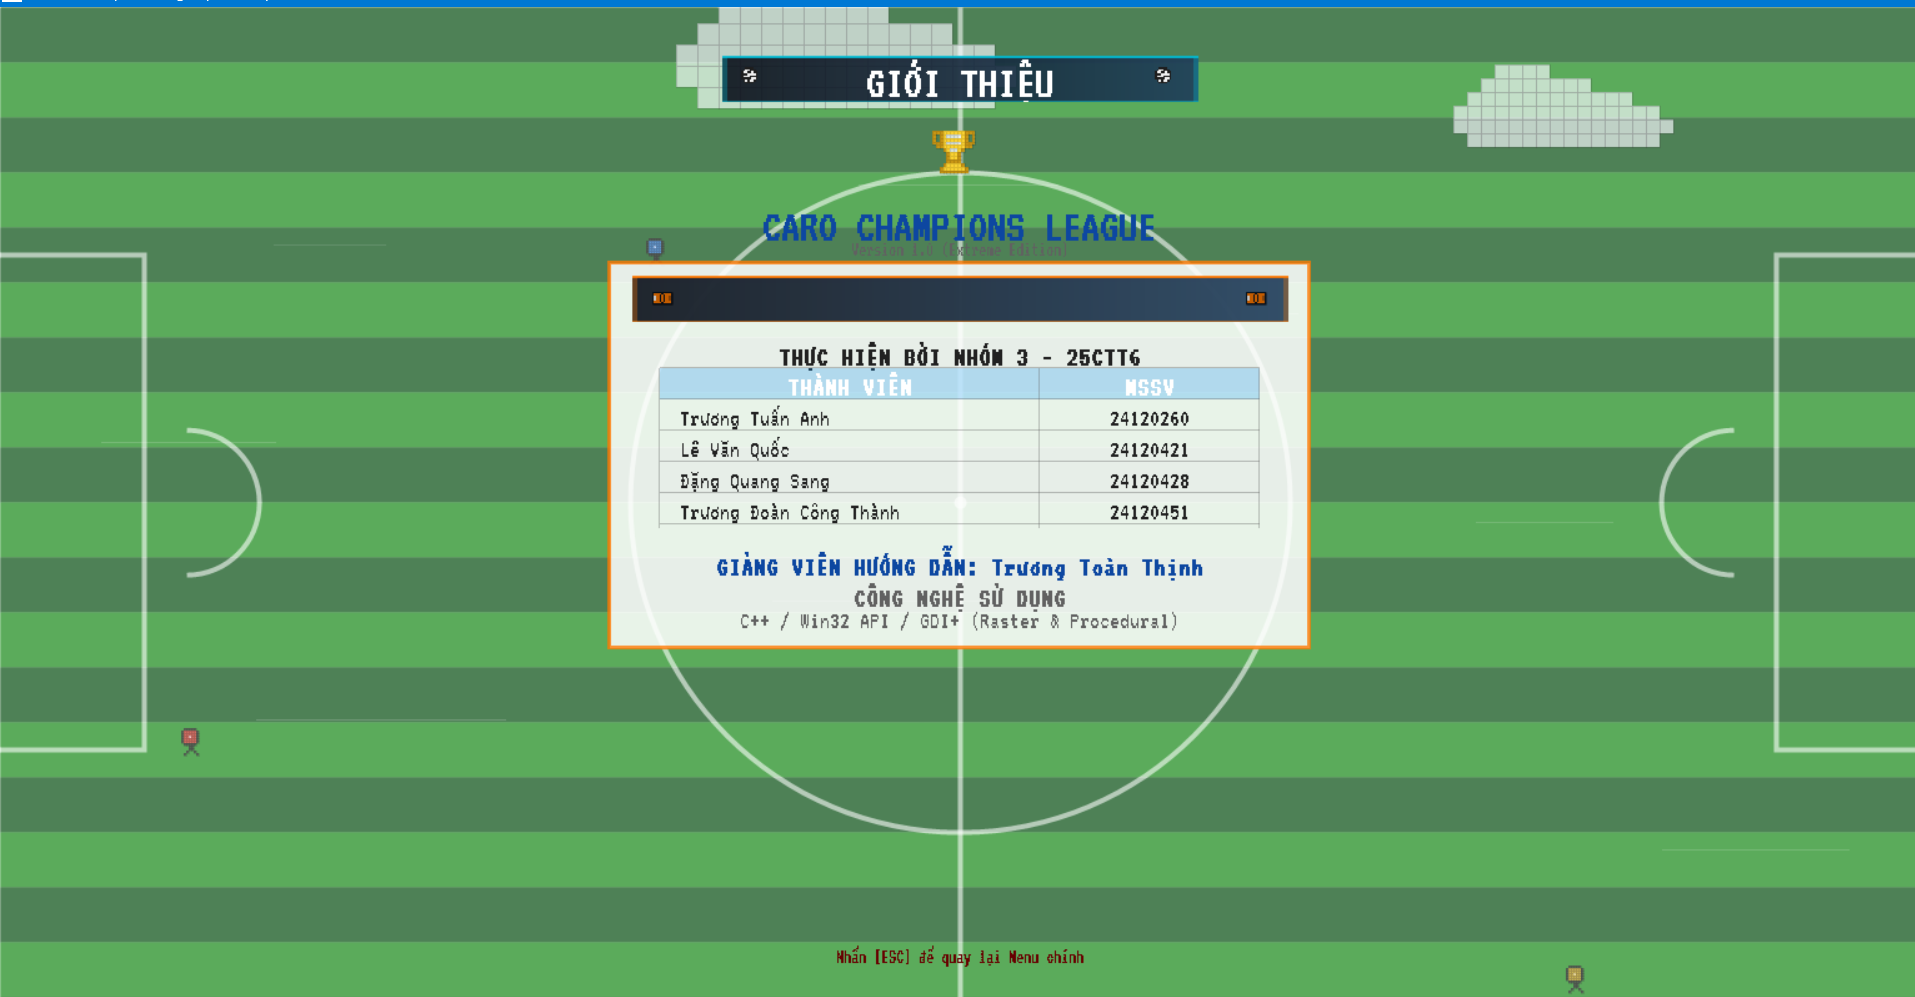
\includegraphics[width=0.9\linewidth]{images/ch4_about.png}
\end{table}

\captionsetup{type=lstlisting}
\renewcommand{\arraystretch}{0.8}
\captionof{lstlisting}{Mã nguồn RenderAboutScreen: banner va bang thanh vien}\label{lst:ch4_about_render}
\begin{longtable}{|>{\ttfamily\small\color{black}\raggedleft\arraybackslash}p{0.8cm}|>{\ttfamily\small\color{black}\arraybackslash}p{0.85\linewidth}|}
\hline
\normalfont\bfseries STT & \normalfont\bfseries Mã nguồn \\ \hline
1 & \cppkw{void} RenderAboutScreen(\cpptype{HDC} hdc, \cppkw{int} screenWidth, \cppkw{int} screenHeight) \\ \hline
2 & \{ \\ \hline
3 & \ \ Gdiplus::Graphics g(hdc); \\ \hline
4 & \ \ DrawProceduralStadium(g, screenWidth, screenHeight); \\ \hline
5 & \ \ DrawPixelBanner(g, hdc, GetText("about\_title").c\_str(), screenWidth / 2, UIScaler::SY(80), UIScaler::SX(500), ToCOLORREF(Palette::White), ToCOLORREF(Palette::CyanNormal)); \\ \hline
6 &  \\ \hline
7 & \ \ \cppkw{int} tableW = UIScaler::SX(600); \\ \hline
8 & \ \ \cppkw{int} tableH = UIScaler::SY(175); \\ \hline
9 & \ \ \cppkw{int} tableX = (screenWidth - tableW) / 2; \\ \hline
10 & \ \ \cppkw{int} tableY = UIScaler::SY(395); \\ \hline
11 & \ \ Gdiplus::Pen gridPen(Gdiplus::Color(100, 100, 100, 100), 1.0f); \\ \hline
12 & \ \ g.DrawLine(\&gridPen, (INT)tableX, (INT)tableY, (INT)(tableX + tableW), (INT)tableY); \\ \hline
13 & \} \\ \hline
\end{longtable}

\subsection*{4.6.8. GuildScreen}
\addcontentsline{toc}{subsection}{\textcolor{black}{4.6.8. GuildScreen}}

\setlength{\parindent}{1.5em} GuildScreen chia thành 3 trang hướng dẫn, có chấm phân trang và mũi tên điều hướng:
\begin{itemize}
  \item Trang 1: so sánh Caro và TicTacToe (hai cột).
  \item Trang 2: hướng dẫn di chuyển và thao tác.
  \item Trang 3: giải thích hệ thống AI, thời gian, mục tiêu, lưu trận.
\end{itemize}
\setlength{\parindent}{1.5em} Điểm nhấn UX là phân trang bằng dot + aura, giúp người dùng biết mình đang ở đâu trong chuỗi hướng dẫn.

\setlength{\parindent}{1.5em} Tiêu đề và màu banner thay đổi theo trang (cam, cyan, xanh lá), đồng thời hệ thống hiển thị mũi tên điều hướng ở hai bên để gợi ý thao tác.

\begin{table}[H]
\caption*{Hình 4.11: Hình minh họa GuildScreen}
\addcontentsline{lof}{figure}{Hình 4.11: Hình minh họa GuildScreen}
\centering
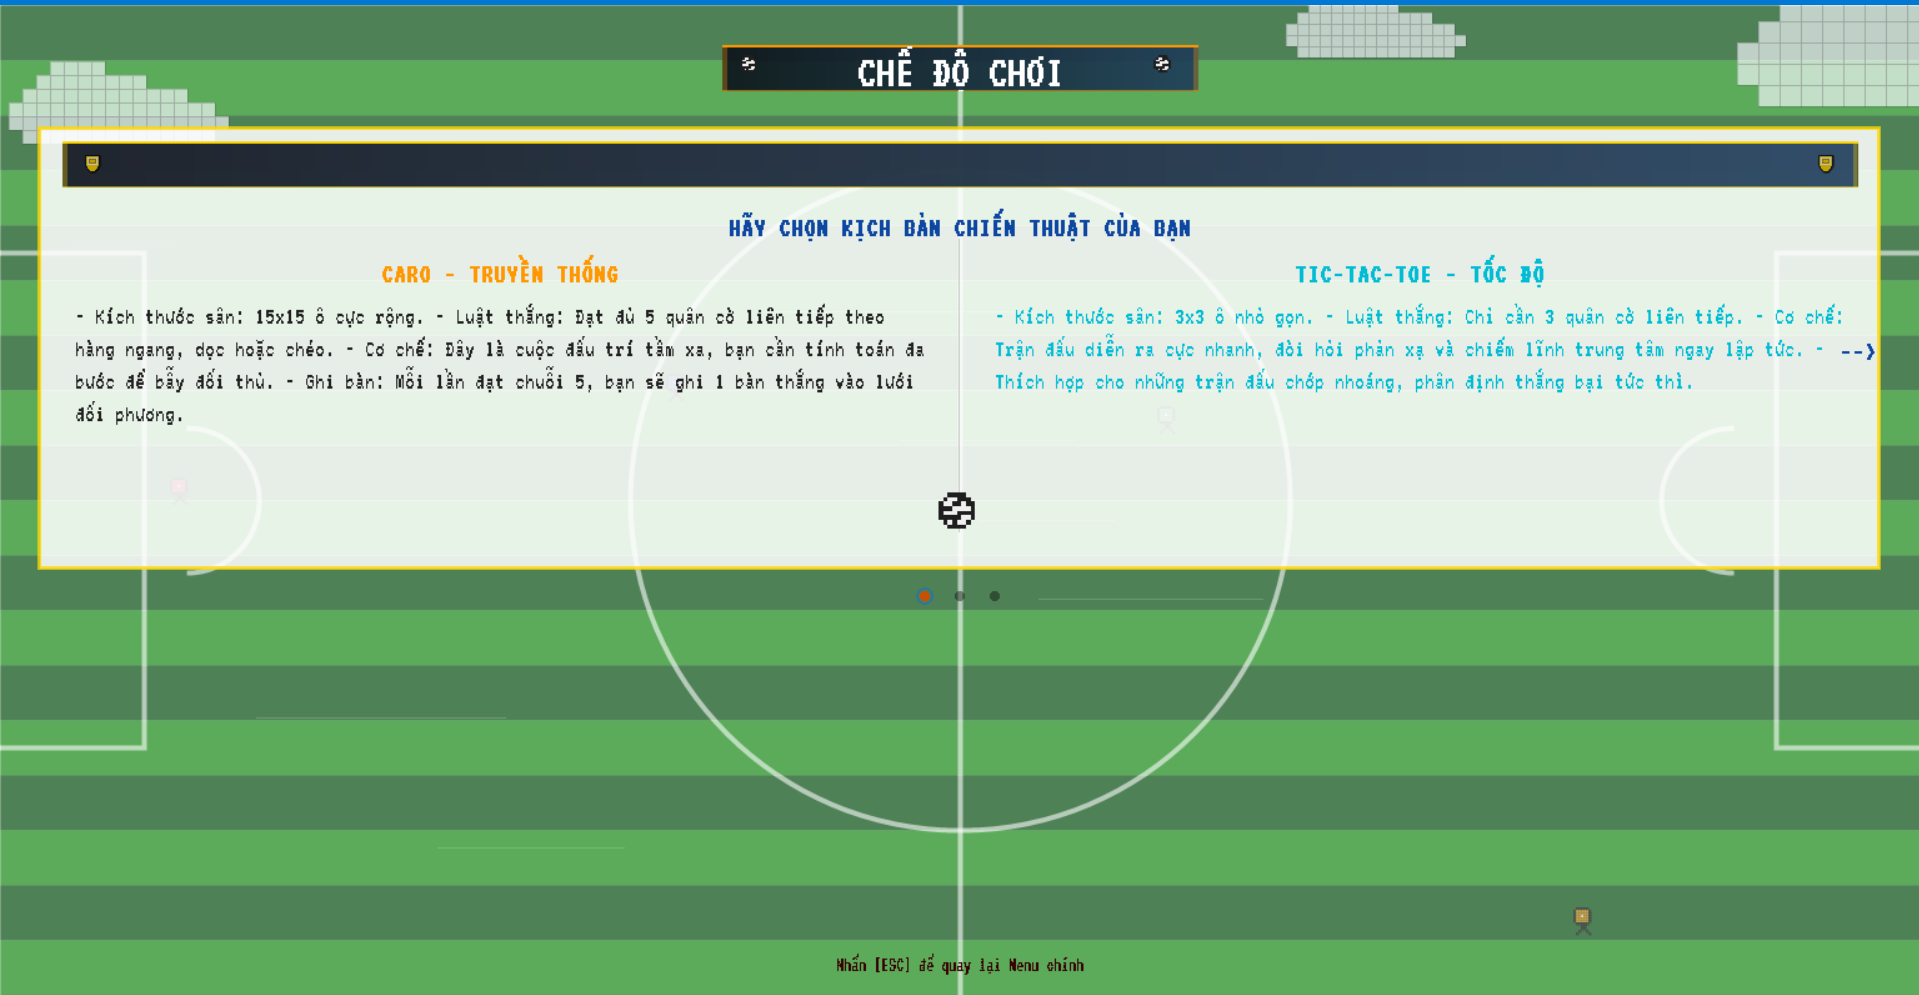
\includegraphics[width=0.9\linewidth]{images/ch4_guild.png}
\end{table}

\captionsetup{type=lstlisting}
\renewcommand{\arraystretch}{0.8}
\captionof{lstlisting}{Mã nguồn RenderGuildScreen: banner va phan trang}\label{lst:ch4_guild_render}
\begin{longtable}{|>{\ttfamily\small\color{black}\raggedleft\arraybackslash}p{0.8cm}|>{\ttfamily\small\color{black}\arraybackslash}p{0.85\linewidth}|}
\hline
\normalfont\bfseries STT & \normalfont\bfseries Mã nguồn \\ \hline
1 & \cppkw{void} RenderGuildScreen(\cpptype{HDC} hdc, \cppkw{int} screenWidth, \cppkw{int} screenHeight, \cppkw{int} currentPage) \\ \hline
2 & \{ \\ \hline
3 & \ \ Gdiplus::Graphics g(hdc); \\ \hline
4 & \ \ DrawProceduralStadium(g, screenWidth, screenHeight); \\ \hline
5 & \ \ COLORREF bannerColors[] = \{ ToCOLORREF(Palette::OrangeNormal), ToCOLORREF(Palette::CyanNormal), ToCOLORREF(Palette::GreenNormal) \}; \\ \hline
6 & \ \ std::wstring titles[] = \{ GetText("guild\_tab1"), GetText("guild\_tab2"), GetText("guild\_tab3") \}; \\ \hline
7 & \ \ DrawPixelBanner(g, hdc, titles[currentPage].c\_str(), screenWidth / 2, UIScaler::SY(70), UIScaler::SX(500), ToCOLORREF(Palette::White), bannerColors[currentPage]); \\ \hline
8 & \} \\ \hline
\end{longtable}

\subsection*{4.6.9. SaveGameScreen}
\addcontentsline{toc}{subsection}{\textcolor{black}{4.6.9. SaveGameScreen}}

\setlength{\parindent}{1.5em} SaveGameScreen có layout tương tự LoadGameScreen nhưng ưu tiên thao tác ghi dữ liệu. Màn hình chia thành ba vùng: danh sách slot, thông tin slot đang chọn, và vùng nhập tên bản lưu. UX mục tiêu là giảm thao tác nhầm: slot trống sẽ hiển thị nhãn "Empty" rõ ràng, slot đã có sẽ hiển thị tên + thời gian lưu gần nhất.

\setlength{\parindent}{1.5em} Khung nhập tên dùng \texttt{Theme::SaveBoxBorder} để tạo viền cam, giúp người chơi nhận biết vùng focus. Tên được giới hạn độ dài ở tầng lưu dữ liệu, nên UI có thể hiển thị thông báo nếu vượt quá giới hạn mà không làm lỗi file.

\setlength{\parindent}{1.5em} Ở chế độ nhập tên, vùng input được tô viền nổi và con trỏ nhấp nháy, đảm bảo người chơi nhận biết trạng thái đang nhập. Khi lưu thành công, thông báo trạng thái hiển thị ngắn ở góc dưới để xác nhận mà không phá bố cục.

\begin{figure}[H]
  \addcontentsline{lof}{figure}{Hình 4.12: Hình minh họa SaveGameScreen}
\centering
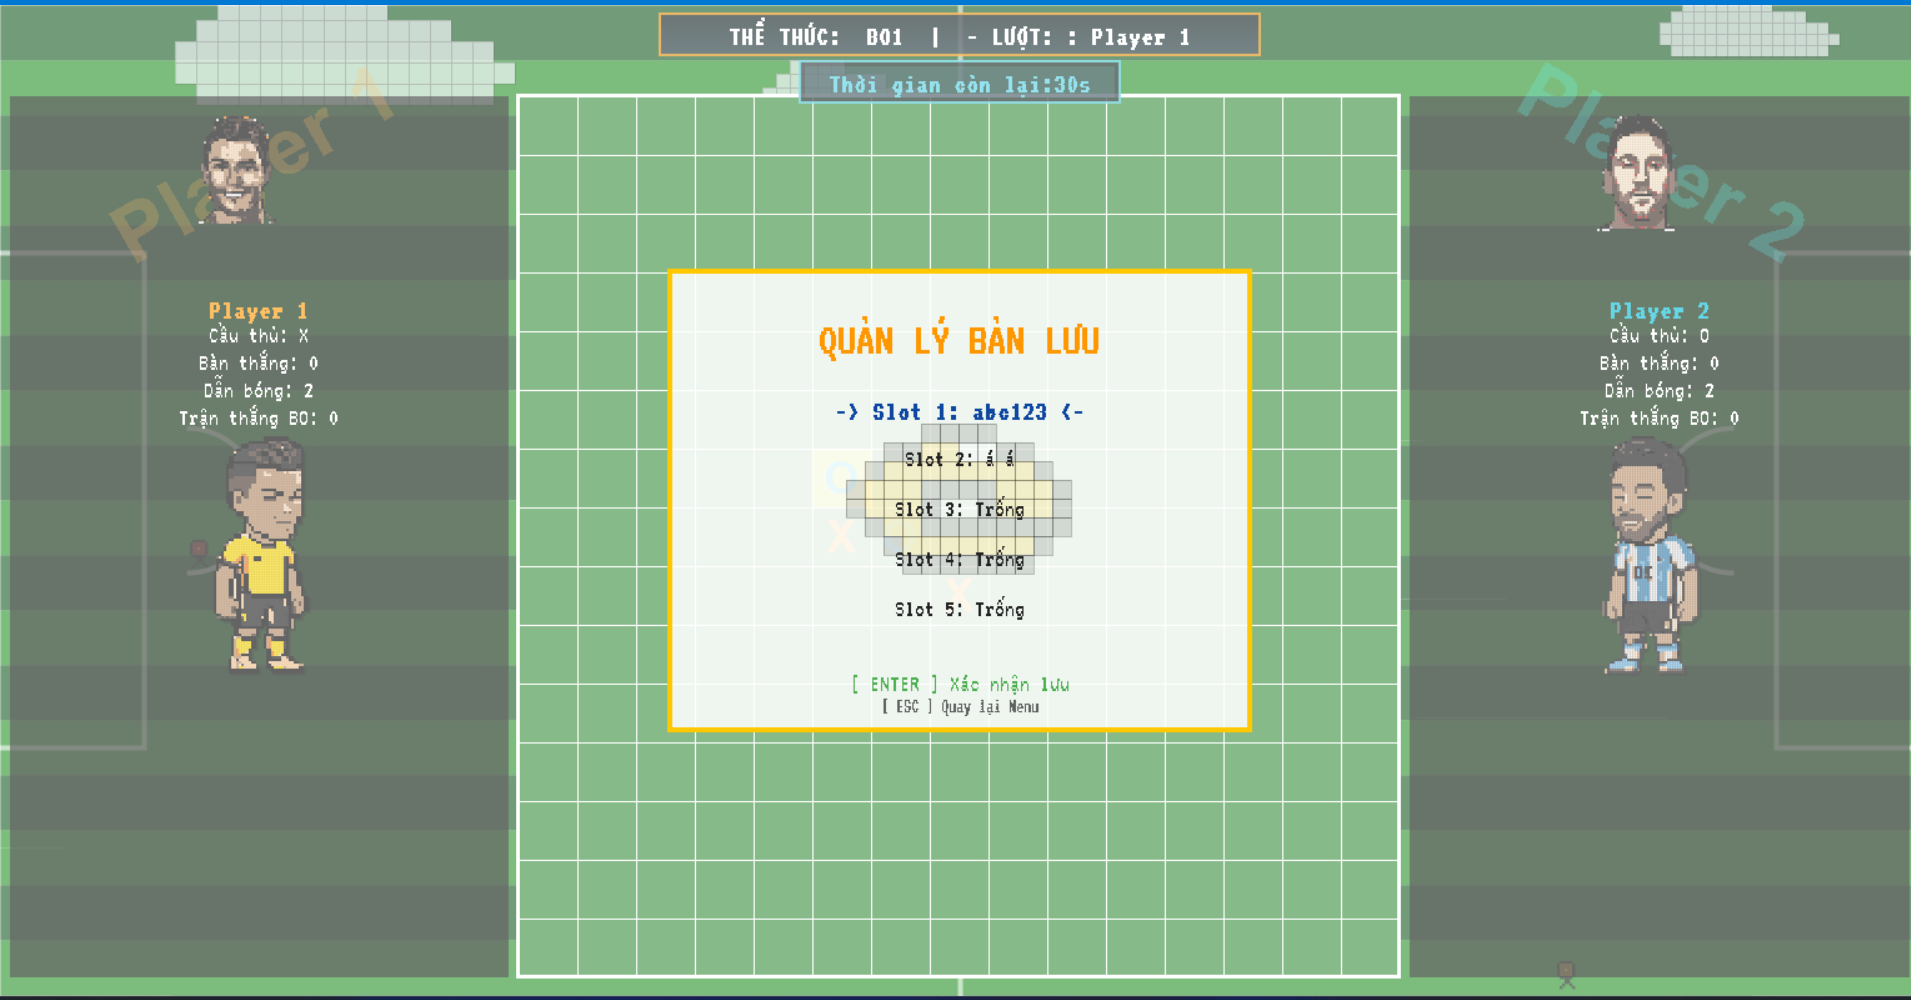
\includegraphics[width=0.45\linewidth]{images/ch4_save_game.png}
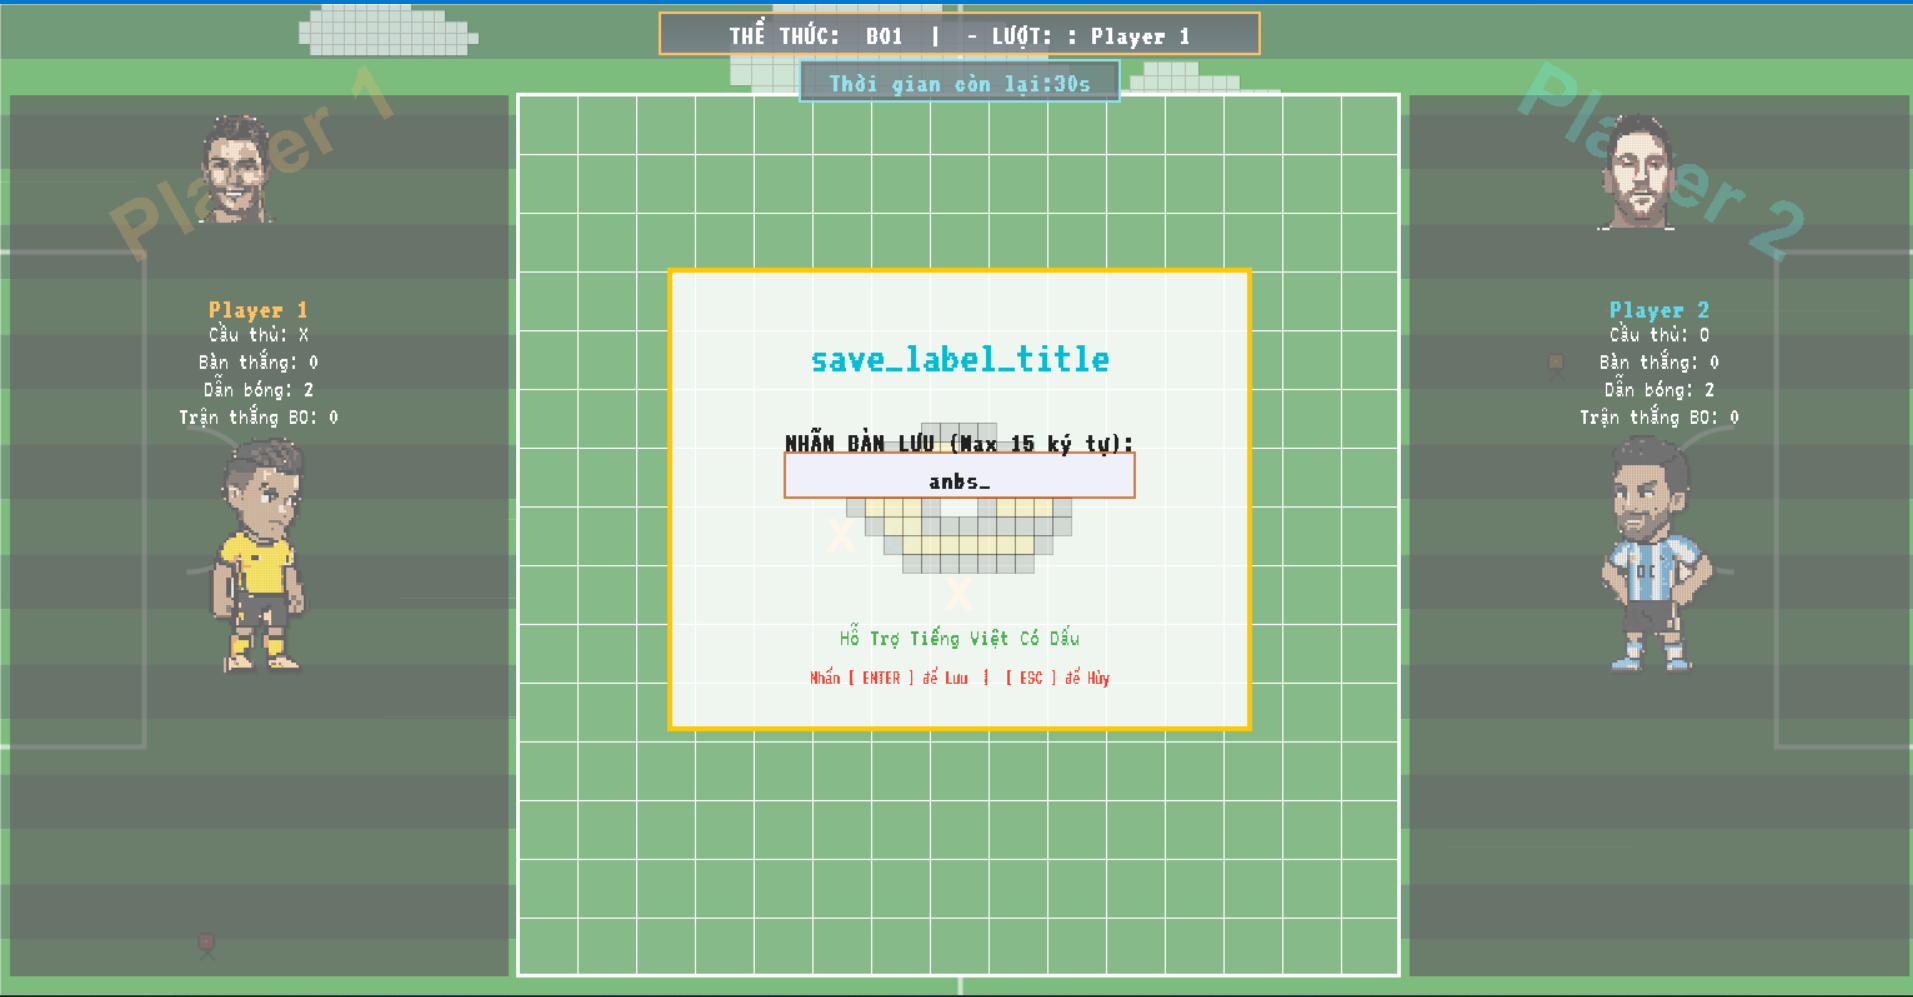
\includegraphics[width=0.45\linewidth]{images/ch4_save_game_2.png}
\caption*{Hình 4.12: Hình minh họa SaveGameScreen}
\end{figure}

\captionsetup{type=lstlisting}
\renewcommand{\arraystretch}{0.8}
\captionof{lstlisting}{Mã nguồn RenderSaveGameScreen: bố cục và banner}\label{lst:ch4_save_render}
\begin{longtable}{|>{\ttfamily\small\color{black}\raggedleft\arraybackslash}p{0.8cm}|>{\ttfamily\small\color{black}\arraybackslash}p{0.85\linewidth}|}
\hline
\normalfont\bfseries STT & \normalfont\bfseries Mã nguồn \\ \hline
1 & \cppkw{void} RenderSaveGameScreen(\cpptype{HDC} hdc, \cppkw{int} selectedOption, \cppkw{const} \cpptype{std::wstring} \&statusMessage, \cppkw{int} screenWidth, \cppkw{int} screenHeight) \\ \hline
2 & \{ \\ \hline
3 & \ \ Gdiplus::Graphics g(hdc); \\ \hline
4 & \ \ DrawProceduralStadium(g, screenWidth, screenHeight); \\ \hline
5 & \ \ \cppkw{int} panelW = UIScaler::SX(900); \\ \hline
6 & \ \ \cppkw{int} panelH = UIScaler::SY(540); \\ \hline
7 & \ \ \cppkw{int} panelX = (screenWidth - panelW) / 2; \\ \hline
8 & \ \ \cppkw{int} panelY = (screenHeight - panelH) / 2; \\ \hline
9 & \ \ Gdiplus::SolidBrush bgBrush(ToGdiColor(Theme::GlassWhite)); \\ \hline
10 & \ \ g.FillRectangle(\&bgBrush, panelX, panelY, panelW, panelH); \\ \hline
11 & \ \ DrawPixelBanner(g, hdc, GetText("save\_title").c\_str(), screenWidth / 2, panelY + UIScaler::SY(45), panelW - UIScaler::SX(40), ToCOLORREF(Palette::White), RGB(0, 150, 255), "Asset/models/bg/cassette.txt"); \\ \hline
12 & \} \\ \hline
\end{longtable}

\subsection*{4.6.10. SummaryScreen}
\addcontentsline{toc}{subsection}{\textcolor{black}{4.6.10. SummaryScreen}}

\setlength{\parindent}{1.5em} SummaryScreen là màn hình tổng kết sau ván/series, tập trung hiển thị thông tin cốt lõi: người thắng, tỷ số, thời gian, và các nút hành động (chơi lại, về menu). UI dùng banner màu nổi và hiệu ứng glow theo màu người thắng để nhấn mạnh kết quả.

\setlength{\parindent}{1.5em} Các màu victory banner và highlight kết quả lấy theo Theme (\texttt{P1TurnBorder} hoặc \texttt{P2TurnBorder}), nên người chơi nhận biết nhanh bên thắng mà không cần đọc chữ.

\setlength{\parindent}{1.5em} Phần số liệu được căn giữa theo chiều dọc, dùng font lớn để đảm bảo đọc nhanh. Các nút điều hướng được bố trí dưới cùng và tách biệt bằng khoảng đệm lớn để tránh bấm nhầm.

\begin{table}[H]
\caption*{Hình 4.13: Hình minh họa SummaryScreen}
\addcontentsline{lof}{figure}{Hình 4.13: Hình minh họa SummaryScreen}
\centering
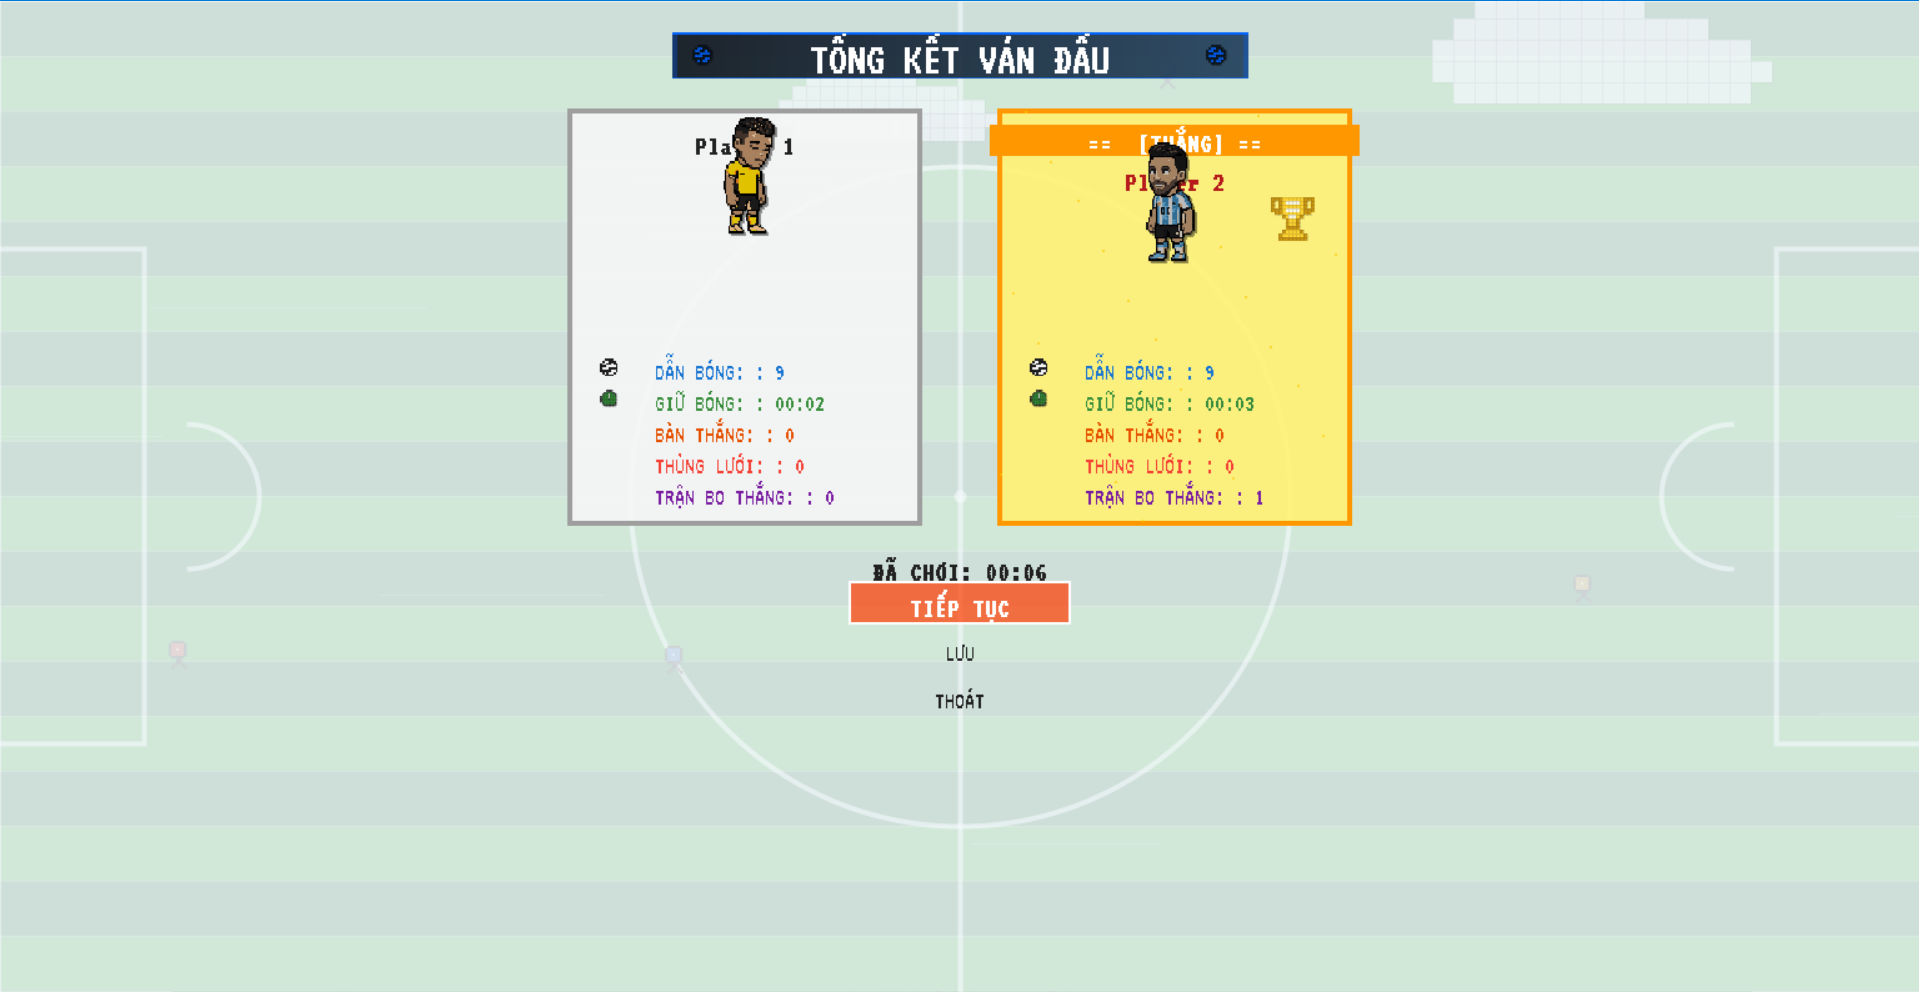
\includegraphics[width=0.9\linewidth]{images/ch4_summary.png}
\end{table}

\captionsetup{type=lstlisting}
\renewcommand{\arraystretch}{0.8}
\captionof{lstlisting}{Mã nguồn RenderSummaryScreen: banner và vùng kết quả}\label{lst:ch4_summary_render}
\begin{longtable}{|>{\ttfamily\small\color{black}\raggedleft\arraybackslash}p{0.8cm}|>{\ttfamily\small\color{black}\arraybackslash}p{0.85\linewidth}|}
\hline
\normalfont\bfseries STT & \normalfont\bfseries Mã nguồn \\ \hline
1 & \cppkw{void} RenderSummaryScreen(\cpptype{HDC} hdc, \cppkw{const} \cpptype{PlayState} *state, \cppkw{int} screenWidth, \cppkw{int} screenHeight) \\ \hline
2 & \{ \\ \hline
3 & \ \ Gdiplus::Graphics g(hdc); \\ \hline
4 & \ \ DrawProceduralStadium(g, screenWidth, screenHeight); \\ \hline
5 & \ \ \cppkw{int} panelW = UIScaler::SX(800); \\ \hline
6 & \ \ \cppkw{int} panelH = UIScaler::SY(420); \\ \hline
7 & \ \ \cppkw{int} panelX = (screenWidth - panelW) / 2; \\ \hline
8 & \ \ \cppkw{int} panelY = (screenHeight - panelH) / 2; \\ \hline
9 & \ \ Gdiplus::SolidBrush bgBrush(ToGdiColor(Theme::GlassWhite)); \\ \hline
10 & \ \ g.FillRectangle(\&bgBrush, panelX, panelY, panelW, panelH); \\ \hline
11 & \ \ DrawPixelBanner(g, hdc, GetText("summary\_title").c\_str(), screenWidth / 2, panelY + UIScaler::SY(45), panelW - UIScaler::SX(40), ToCOLORREF(Palette::White), RGB(255, 180, 0), "Asset/models/bg/trophy.txt"); \\ \hline
12 & \} \\ \hline
\end{longtable}

\section*{4.7. Tối ưu hóa và quản lý tài nguyên}
\addcontentsline{toc}{section}{\textcolor{black}{4.7. Tối ưu hóa và quản lý tài nguyên}}

\setlength{\parindent}{1.5em} Hệ thống có cơ chế dọn cache tập trung để tránh rò rỉ bộ nhớ. Hàm \texttt{ClearUICaches} giải phóng toàn bộ bitmap cache và brush cache khi cần (ví dụ khi đổi độ phân giải lớn hoặc thoát game).

\setlength{\parindent}{1.5em} Hàm này dọn tuần tự từng nhóm cache (model, avatar, football, trophy, clock, action, brush). Việc dọn theo nhóm giúp tránh bỏ sót và đảm bảo bộ nhớ đồ họa không bị giữ lại sau khi đổi scene lớn hoặc khi tắt game.

\captionsetup{type=lstlisting}
\renewcommand{\arraystretch}{0.8}
\captionof{lstlisting}{Mã nguồn Dọn cache UI tập trung}\label{lst:ch4_clear_caches}
\begin{longtable}{|>{\ttfamily\small\color{black}\raggedleft\arraybackslash}p{0.8cm}|>{\ttfamily\small\color{black}\arraybackslash}p{0.85\linewidth}|}
\hline
\normalfont\bfseries STT & \normalfont\bfseries Mã nguồn \\ \hline
1 & \cppkw{void} ClearUICaches() \\ \hline
2 & \{ \\ \hline
3 & \ \ \cppkw{for} (\cppkw{auto} \&pair : g\_ModelCache) \{ \cppkw{if} (pair.second) \cppkw{delete} pair.second; \} \\ \hline
4 & \ \ g\_ModelCache.clear(); \\ \hline
5 &  \\ \hline
6 & \ \ \cppkw{for} (\cppkw{auto} \&pair : g\_AvatarCache) \{ \cppkw{if} (pair.second) \cppkw{delete} pair.second; \} \\ \hline
7 & \ \ g\_AvatarCache.clear(); \\ \hline
8 &  \\ \hline
9 & \ \ \cppkw{for} (\cppkw{auto} \&pair : g\_BrushCache) \{ \cppkw{if} (pair.second) \cppkw{delete} pair.second; \} \\ \hline
10 & \ \ g\_BrushCache.clear(); \\ \hline
11 & \} \\ \hline
\end{longtable}

\setlength{\parindent}{1.5em} Ngoài ra, mô hình ``data-driven pixel art'' giúp giảm kích thước asset ảnh, đồng thời cho phép thay đổi palette nhanh theo theme mà không cần sửa lại sprite.

\section*{4.8. Vòng lặp ứng dụng và điều phối input}
\addcontentsline{toc}{section}{\textcolor{black}{4.8. Vòng lặp ứng dụng và điều phối input}}

\setlength{\parindent}{1.5em} Phần này mô tả vòng lặp chính của ứng dụng (message pump + update/render) và cơ chế throttling input để tránh spam phím. Hai cơ chế này quyết định tính ổn định FPS và cảm giác điều khiển trong UI.

\subsection*{4.8.1. Message pump, dt và giới hạn bước nhảy thời gian}
\addcontentsline{toc}{subsection}{\textcolor{black}{4.8.1. Message pump, dt và giới hạn bước nhảy thời gian}}

\setlength{\parindent}{1.5em} Vòng lặp chính xử lý toàn bộ tin nhắn đang chờ, sau đó mới chạy update và render. Thời gian khung hình \texttt{dt} được tính từ \texttt{high\_resolution\_clock} và bị chặn ở ngưỡng 0.1s để tránh "nhảy vọt" khi người dùng kéo/di chuyển cửa sổ. Điều này giữ logic ổn định và tránh cập nhật quá lớn gây vỡ animation.

\captionsetup{type=lstlisting}
\renewcommand{\arraystretch}{0.8}
\captionof{lstlisting}{Vòng lặp chính: xử lý message và giới hạn dt}\label{lst:ch4_main_loop}
\begin{longtable}{|>{\ttfamily\small\color{black}\raggedleft\arraybackslash}p{0.8cm}|>{\ttfamily\small\color{black}\arraybackslash}p{0.85\linewidth}|}
\hline
\normalfont\bfseries STT & \normalfont\bfseries Mã nguồn \\ \hline
1 & \cppkw{while} (bRunning) \{ \\ \hline
2 & \ \ \cppkw{while} (PeekMessage(\&msg, NULL, 0, 0, PM\_REMOVE)) \{ \\ \hline
3 & \ \ \ \ \cppkw{if} (msg.message == WM\_QUIT) \{ bRunning = \cppkw{false}; \cppkw{break}; \} \\ \hline
4 & \ \ \ \ TranslateMessage(\&msg); \ DispatchMessage(\&msg); \\ \hline
5 & \ \ \} \\ \hline
6 & \ \ \cppkw{if} (!bRunning) \cppkw{break}; \\ \hline
7 & \ \ \cppkw{auto} frameStart = std::chrono::high\_resolution\_clock::now(); \\ \hline
8 & \ \ std::chrono::duration<double> elapsed = frameStart - lastTime; \\ \hline
9 & \ \ lastTime = frameStart; \\ \hline
10 & \ \ \cppkw{double} dt = elapsed.count(); \\ \hline
11 & \ \ \cppkw{if} (dt > 0.1) dt = 0.1; \\ \hline
12 & \ \ g\_GlobalAnimTime += (float)dt; \\ \hline
13 & \} \\ \hline
\end{longtable}

\subsection*{4.8.2. Throttling input và chống autorepeat quá nhanh}
\addcontentsline{toc}{subsection}{\textcolor{black}{4.8.2. Throttling input và chống autorepeat quá nhanh}}

\setlength{\parindent}{1.5em} Ở menu và các màn hình điều hướng, phím di chuyển được giới hạn tốc độ để tránh "nhảy" nhiều mục khi người dùng giữ phím. Hệ thống tách nhấn thường và autorepeat, áp dụng ngưỡng 80ms cho nhấn tay và 150ms cho phím giữ. Cách này giữ cảm giác điều khiển mượt và dễ kiểm soát.

\captionsetup{type=lstlisting}
\renewcommand{\arraystretch}{0.8}
\captionof{lstlisting}{Throttling phím điều hướng trong MenuScreen}\label{lst:ch4_menu_throttle}
\begin{longtable}{|>{\ttfamily\small\color{black}\raggedleft\arraybackslash}p{0.8cm}|>{\ttfamily\small\color{black}\arraybackslash}p{0.85\linewidth}|}
\hline
\normalfont\bfseries STT & \normalfont\bfseries Mã nguồn \\ \hline
1 & \cppkw{bool} isRepeat = (wParam \& 0x20000) != 0; \\ \hline
2 & WPARAM rawKey = wParam \& 0xFFFF; \\ \hline
3 & \cppkw{static} ULONGLONG lastMoveTime = 0; \\ \hline
4 & ULONGLONG now = GetTickCount64(); \\ \hline
5 & \cppkw{bool} canMove = (now - lastMoveTime > (ULONGLONG)(isRepeat ? 150 : 80)); \\ \hline
6 & \cppkw{if} (rawKey == 'W' || rawKey == 'w' || rawKey == VK\_UP) \{ \\ \hline
7 & \ \ \cppkw{if} (!canMove) \cppkw{return} \cppkw{false}; \\ \hline
8 & \ \ selectedOption--; \\ \hline
9 & \ \ \cppkw{if} (!isRepeat) PlaySFX("sfx\_move"); \\ \hline
10 & \ \ lastMoveTime = now; \\ \hline
11 & \} \\ \hline
\end{longtable}
